\documentclass[9pt,xcolor={table}]{beamer}
\setbeamertemplate{caption}[numbered]
\usetheme[white]{Illinois}
%\title[short title]{long title}
\title[HALEU Transitions]{Investigation of Impacts of Deploying 
Reactors Fueled by High Assay Low Enriched Uranium}
\subtitle{Final Defense}
\author[Amanda M. Bachmann]{Amanda M. Bachmann\\ Advanced Reactors and Fuel Cycles Group}
%\author[Kathryn D. Huff]{Kathryn D. Huff\\Advanced Reactors and Fuel Cycles Group}
\date[11.02.2023]{November 2, 2023}
\institute[UIUC]{University of Illinois at Urbana-Champaign}


\usepackage[table]{xcolor}
\usepackage{amsfonts}
\usepackage{amsmath}
\usepackage{xspace}
\usepackage{graphicx}
\usepackage{caption}
\usepackage{subcaption}
\usepackage{booktabs} % nice rules for tables
\usepackage{microtype} % if using PDF
\usepackage{bigints}
\usepackage{array}
\newcolumntype{x}[1]{>{\centering\arraybackslash\hspace{0pt}}p{#1}}

\usepackage{threeparttable}

\graphicspath{{../images/}}

\newcommand{\units}[1] {\:\text{#1}}%
\newcommand{\SN}{S$_N$}%{S$_\text{N}$}%{$S_N$}%
\newcommand{\Cyclus}{\textsc{Cyclus}\xspace} %
\newcommand{\Cycamore}{\textsc{Cycamore}\xspace} %
\newcommand{\keff}{$k_{eff}$\xspace}
\newcommand{\betaEff}{$\beta_{eff}$\xspace}
\DeclareMathOperator{\erf}{erf}
%I need some complimentary error functions... 
\DeclareMathOperator{\erfc}{erfc}
%Those icons in the references are terrible looking
\setbeamertemplate{bibliography item}[text]

%%%% Acronym support

\usepackage[acronym,toc]{glossaries}
\newacronym[longplural={metric tons of heavy metal}]{MTHM}{MTHM}{metric ton of heavy metal}
\newacronym{ABM}{ABM}{agent-based modeling}
\newacronym{ACDIS}{ACDIS}{Program in Arms Control \& Domestic and International Security}
\newacronym{AFCI}{AFCI}{Advanced Fuel Cycle Initiative}
\newacronym{AHTR}{AHTR}{Advanced High Temperature Reactor}
\newacronym{ANDRA}{ANDRA}{Agence Nationale pour la gestion des D\'echets RAdioactifs, the French National Agency for Radioactive Waste Management}
\newacronym{ANL}{ANL}{Argonne National Laboratory}
\newacronym{ARDP}{ARDP}{Advanced Reactors Demonstration Program}
\newacronym{API}{API}{application programming interface}
\newacronym{ARCH}{ARCH}{autoregressive conditional heteroskedastic}
\newacronym{ARE}{ARE}{Aircraft Reactor Experiment}
\newacronym{ARFC}{ARFC}{Advanced Reactors and Fuel Cycles}
\newacronym{ARMA}{ARMA}{autoregressive moving average}
\newacronym{ASME}{ASME}{American Society of Mechanical Engineers}
\newacronym{ATWS}{ATWS}{Anticipated Transient Without Scram}
\newacronym{BDBE}{BDBE}{Beyond Design Basis Event}
\newacronym{BIDS}{BIDS}{Berkeley Institute for Data Science}
\newacronym{BOL}{BOL}{Beginning-of-Life}
\newacronym{BSD}{BSD}{Berkeley Software Distribution}
\newacronym{BWR}{BWR}{Boiling Water Reactor}
\newacronym{CAFCA}{CAFCA}{ Code for Advanced Fuel Cycles Assessment }
\newacronym{CASL}{CASL}{Consortium for Advanced Simulation of Light Water Reactors}
\newacronym{CDTN}{CDTN}{Centro de Desenvolvimento da Tecnologia Nuclear}
\newacronym{CEA}{CEA}{Commissariat \`a l'\'Energie Atomique et aux \'Energies Alternatives}
\newacronym{CF}{CF}{capacity factor}
\newacronym{CI}{CI}{continuous integration}
\newacronym{CNEC}{CNEC}{Consortium for Nonproliferation Enabling Capabilities}
\newacronym{CNEN}{CNEN}{Comiss\~{a}o Nacional de Energia Nuclear}
\newacronym{CNERG}{CNERG}{Computational Nuclear Engineering Research Group}
\newacronym{COSI}{COSI}{Commelini-Sicard}
\newacronym{COTS}{COTS}{commercial, off-the-shelf}
\newacronym{CSNF}{CSNF}{commercial spent nuclear fuel}
\newacronym{CTAH}{CTAHs}{Coiled Tube Air Heaters}
\newacronym{CUBIT}{CUBIT}{CUBIT Geometry and Mesh Generation Toolkit}
\newacronym{CURIE}{CURIE}{Centralized Used Fuel Resource for Information Exchange}
\newacronym{DAG}{DAG}{directed acyclic graph}
\newacronym{DANESS}{DANESS}{Dynamic Analysis of Nuclear Energy System Strategies}
\newacronym{DBE}{DBE}{Design Basis Event}
\newacronym{DESAE}{DESAE}{Dynamic Analysis of Nuclear Energy Systems Strategies}
\newacronym{DHS}{DHS}{Department of Homeland Security}
\newacronym{DOE}{DOE}{Department of Energy}
\newacronym{DOE-NE}{DOE-NE}{U.S. Department of Energy, Office of Nuclear Energy}
\newacronym{DRACS}{DRACS}{Direct Reactor Auxiliary Cooling System}
\newacronym{DRE}{DRE}{dynamic resource exchange}
\newacronym{DSNF}{DSNF}{DOE spent nuclear fuel}
\newacronym{DYMOND}{DYMOND}{Dynamic Model of Nuclear Development }
\newacronym{EBS}{EBS}{Engineered Barrier System}
\newacronym{EBR}{EBR-II}{Experimental Breeder Reactor II}
\newacronym{EDZ}{EDZ}{Excavation Disturbed Zone}
\newacronym{EG}{EG}{Evaluation Group}
\newacronym{EIA}{EIA}{U.S. Energy Information Administration}
\newacronym{EOL}{EOL}{End-of-life}
\newacronym{EPA}{EPA}{Environmental Protection Agency}
\newacronym{EP}{EP}{Engineering Physics}
\newacronym{ES}{E\&S}{Evaluation and Screening}
\newacronym{FCM}{FCM}{Fully Ceramic Microencapsulated}
\newacronym{FCO}{FCO}{Fuel Cycle Options}
\newacronym{FCT}{FCT}{Fuel Cycle Technology}
\newacronym{FCWMD}{FCWMD}{Fuel Cycle and Waste Management Division}
\newacronym{FEHM}{FEHM}{Finite Element Heat and Mass Transfer}
\newacronym{FEPs}{FEPs}{Features, Events, and Processes}
\newacronym{FHR}{FHR}{Fluoride-Salt-Cooled High-Temperature Reactor}
\newacronym{FLiBe}{FLiBe}{Fluoride-Lithium-Beryllium}
\newacronym{GCAM}{GCAM}{Global Change Assessment Model}
\newacronym{GDSE}{GDSE}{Generic Disposal System Environment}
\newacronym{GDSM}{GDSM}{Generic Disposal System Model}
\newacronym{GENIUSv1}{GENIUSv1}{Global Evaluation of Nuclear Infrastructure Utilization Scenarios, Version 1}
\newacronym{GENIUSv2}{GENIUSv2}{Global Evaluation of Nuclear Infrastructure Utilization Scenarios, Version 2}
\newacronym{GENIUS}{GENIUS}{Global Evaluation of Nuclear Infrastructure Utilization Scenarios}
\newacronym{GPAM}{GPAM}{Generic Performance Assessment Model}
\newacronym{GRSAC}{GRSAC}{Graphite Reactor Severe Accident Code}
\newacronym{GUI}{GUI}{graphical user interface}
\newacronym{HALEU}{HALEU}{High Assay Low Enriched Uranium}
\newacronym{HEU}{HEU}{High Enriched Uranium}
\newacronym{HLW}{HLW}{high level waste}
\newacronym{HPC}{HPC}{high-performance computing}
\newacronym{HTC}{HTC}{high-throughput computing}
\newacronym{HTGR}{HTGR}{High Temperature Gas-Cooled Reactor}
\newacronym{HTTR}{HTTR}{High Temperature Engineering Test Reactor}
\newacronym{IAEA}{IAEA}{International Atomic Energy Agency}
\newacronym{IEMA}{IEMA}{Illinois Emergency Mangament Agency}
\newacronym{INL}{INL}{Idaho National Laboratory}
\newacronym{IPRR1}{IRP-R1}{Instituto de Pesquisas Radioativas Reator 1}
\newacronym{IRP}{IRP}{Integrated Research Project}
\newacronym{ISFSI}{ISFSI}{Independent Spent Fuel Storage Installation}
\newacronym{ISRG}{ISRG}{Independent Student Research Group}
\newacronym{JFNK}{JFNK}{Jacobian-Free Newton Krylov}
\newacronym{LANL}{LANL}{Los Alamos National Laboratory}
\newacronym{LBNL}{LBNL}{Lawrence Berkeley National Laboratory}
\newacronym{LCOE}{LCOE}{levelized cost of electricity}
\newacronym{LDRD}{LDRD}{laboratory directed research and development}
\newacronym{LEU}{LEU}{Low Enriched Uranium}
\newacronym{LFR}{LFR}{Lead-Cooled Fast Reactor}
\newacronym{LGPL}{LGPL}{Lesser GNU Public License}
\newacronym{LLNL}{LLNL}{Lawrence Livermore National Laboratory}
\newacronym{LLW}{LLW}{low level waste}
\newacronym{LMFBR}{LMFBR}{Liquid-Metal-cooled Fast Breeder Reactor}
\newacronym{LOFC}{LOFC}{Loss of Forced Cooling}
\newacronym{LOHS}{LOHS}{Loss of Heat Sink}
\newacronym{LOLA}{LOLA}{Loss of Large Area}
\newacronym{LP}{LP}{linear program}
\newacronym{LWR}{LWR}{Light Water Reactor}
\newacronym{MARKAL}{MARKAL}{MARKet and ALlocation}
\newacronym{MA}{MA}{minor actinide}
\newacronym{MCNP}{MCNP}{Monte Carlo N-Particle code}
\newacronym{MILP}{MILP}{mixed-integer linear program}
\newacronym{MIT}{MIT}{the Massachusetts Institute of Technology}
\newacronym{MMR}{MMR}{Micro Modular Reactor}
\newacronym{MOAB}{MOAB}{Mesh-Oriented datABase}
\newacronym{MOOSE}{MOOSE}{Multiphysics Object-Oriented Simulation Environment}
\newacronym{MOX}{MOX}{mixed oxide}
\newacronym{MSBR}{MSBR}{Molten Salt Breeder Reactor}
\newacronym{MSRE}{MSRE}{Molten Salt Reactor Experiment}
\newacronym{MSR}{MSR}{Molten Salt Reactor}
\newacronym{NAGRA}{NAGRA}{National Cooperative for the Disposal of Radioactive Waste}
\newacronym{NCSA}{NCSA}{National Center for Supercomputing Applications}
\newacronym{NEAMS}{NEAMS}{Nuclear Engineering Advanced Modeling and Simulation}
\newacronym{NEUP}{NEUP}{Nuclear Energy University Programs}
\newacronym{NFCSim}{NFCSim}{Nuclear Fuel Cycle Simulator}
\newacronym{NFC}{NFC}{Nuclear Fuel Cycle}
\newacronym{NGNP}{NGNP}{Next Generation Nuclear Plant}
\newacronym{NMWPC}{NMWPC}{Nuclear MW Per Capita}
\newacronym{NNSA}{NNSA}{National Nuclear Security Administration}
\newacronym{NPRE}{NPRE}{Department of Nuclear, Plasma, and Radiological Engineering}
\newacronym{NQA1}{NQA-1}{Nuclear Quality Assurance - 1}
\newacronym{NRC}{NRC}{Nuclear Regulatory Commission}
\newacronym{NSF}{NSF}{National Science Foundation}
\newacronym{NSSC}{NSSC}{Nuclear Science and Security Consortium}
\newacronym{NUWASTE}{NUWASTE}{Nuclear Waste Assessment System for Technical Evaluation}
\newacronym{NWF}{NWF}{Nuclear Waste Fund}
\newacronym{NWTRB}{NWTRB}{Nuclear Waste Technical Review Board}
\newacronym{OAT}{OAT}{one-at-a-time}
\newacronym{OCRWM}{OCRWM}{Office of Civilian Radioactive Waste Management}
\newacronym{OECD}{OECD}{Organisation for Economic Cooperation and Development}
\newacronym{ORION}{ORION}{ORION}
\newacronym{ORNL}{ORNL}{Oak Ridge National Laboratory}
\newacronym{PARCS}{PARCS}{Purdue Advanced Reactor Core Simulator}
\newacronym{PBAHTR}{PB-AHTR}{Pebble Bed Advanced High Temperature Reactor}
\newacronym{PBFHR}{PB-FHR}{Pebble-Bed Fluoride-Salt-Cooled High-Temperature Reactor}
\newacronym{PEI}{PEI}{Peak Environmental Impact}
\newacronym{PH}{PRONGHORN}{PRONGHORN}
\newacronym{PI}{PI}{Principal Investigator}
\newacronym{PNNL}{PNNL}{Pacific Northwest National Laboratory}
\newacronym{PRIS}{PRIS}{Power Reactor Information System}
\newacronym{PRKE}{PRKE}{Point Reactor Kinetics Equations}
\newacronym{PSPG}{PSPG}{Pressure-Stabilizing/Petrov-Galerkin}
\newacronym{PWAR}{PWAR}{Pratt and Whitney Aircraft Reactor}
\newacronym{PWR}{PWR}{Pressurized Water Reactor}
\newacronym{PyNE}{PyNE}{Python toolkit for Nuclear Engineering}
\newacronym{PyRK}{PyRK}{Python for Reactor Kinetics}
\newacronym{QA}{QA}{quality assurance}
\newacronym{RDD}{RD\&D}{Research Development and Demonstration}
\newacronym{RD}{R\&D}{Research and Development}
\newacronym{RELAP}{RELAP}{Reactor Excursion and Leak Analysis Program}
\newacronym{RIA}{RIA}{Reactivity Insertion Accident}
\newacronym{RIF}{RIF}{Region-Institution-Facility}
\newacronym{SAM}{SAM}{Simulation and Modeling}
\newacronym{SCF}{SCF}{Software Carpentry Foundation}
\newacronym{SFR}{SFR}{Sodium-Cooled Fast Reactor}
\newacronym{SINDAG}{SINDA{\textbackslash}G}{Systems Improved Numerical Differencing Analyzer $\backslash$ Gaski}
\newacronym{SKB}{SKB}{Svensk K\"{a}rnbr\"{a}nslehantering AB}
\newacronym{SMR}{SMR}{small modular reactor}
\newacronym{SNF}{SNF}{spent nuclear fuel}
\newacronym{SNL}{SNL}{Sandia National Laboratory}
\newacronym{SNM}{SNM}{Special Nuclear Material}
\newacronym{SRS}{SRS}{Savannah River Site}
\newacronym{STC}{STC}{specific temperature change}
\newacronym{SUPG}{SUPG}{Streamline-Upwind/Petrov-Galerkin}
\newacronym{SWF}{SWF}{Separations and Waste Forms}
\newacronym{SWU}{SWU}{Separative Work Unit}
\newacronym{SandO}{S\&O}{Signatures and Observables}
\newacronym{THW}{THW}{The Hacker Within}
\newacronym{TRIGA}{TRIGA}{Training Research Isotope General Atomic}
\newacronym{TRISO}{TRISO}{Tristructural Isotropic}
\newacronym{TRU}{TRU}{transuranic}
\newacronym{TSM}{TSM}{Total System Model}
\newacronym{TSPA}{TSPA}{Total System Performance Assessment for the Yucca Mountain License Application}
\newacronym{UDB}{UDB}{Unified Database}
\newacronym{UFD}{UFD}{Used Fuel Disposition}
\newacronym{UML}{UML}{Unified Modeling Language}
\newacronym{UNFSTANDARDS}{UNFST\&DARDS}{Used Nuclear Fuel Storage, Transportation \& Disposal Analysis Resource and Data System}
\newacronym{USNC}{USNC}{Ultra Safe Nuclear Company}
\newacronym{UOX}{UOX}{uranium oxide}
\newacronym{UQ}{UQ}{uncertainty quantification}
\newacronym{US}{US}{United States}
\newacronym{UW}{UW}{University of Wisconsin}
\newacronym{VISION}{VISION}{the Verifiable Fuel Cycle Simulation Model}
\newacronym{VV}{V\&V}{verification and validation}
\newacronym{WIPP}{WIPP}{Waste Isolation Pilot Plant}
\newacronym{YMG}{YMG}{Young Members Group}
\newacronym{YMR}{YMR}{Yucca Mountain Repository Site}
\newacronym{NEI}{NEI}{Nuclear Energy Institute}
%\newacronym{<++>}{<++>}{<++>}
%\newacronym{<++>}{<++>}{<++>}

\usepackage{tikz}
\usetikzlibrary{shapes.geometric, arrows, backgrounds}
\usetikzlibrary{positioning, arrows, decorations, shapes, matrix, fit, tikzmark}

\tikzstyle{agent} = [rectangle, rounded corners, minimum width=0.1cm, minimum height=0.2cm,text centered, draw=black, fill=blue!30]
\tikzstyle{transition} = [rectangle, rounded corners, minimum width=0.1cm, minimum height=0.2cm,text centered, draw=black, fill=red!30]
\tikzstyle{arrow} = [thick,->,>=stealth]

\tikzstyle{region} = [rectangle, rounded corners, minimum width=0.1cm, minimum height=0.2cm,text centered, draw=black, fill=green!30]
\tikzstyle{institution} = [rectangle, rounded corners, minimum width=0.1cm, minimum height=0.2cm,text centered, draw=black, fill=red!30]
\tikzstyle{facility} = [rectangle, rounded corners, minimum width=0.1cm, minimum height=0.2cm,text centered, draw=black, fill=blue!30]
\tikzstyle{connect} = [thick,-]

\def\firstcircle{(0,0) circle (2cm)}
\def\secondcircle{(60:3cm) circle (2cm)}
\def\thirdcircle{(0:3cm) circle (2cm)}
\makeglossaries

%try to get rid of header on title page\dots
\makeatletter
    \newenvironment{withoutheadline}{
        \setbeamertemplate{headline}[default]
        \def\beamer@entrycode{\vspace*{-\headheight}}
    }{}
\makeatother

\makeatother
\setbeamertemplate{footline}
{
  \leavevmode%
  \hbox{%
    \rightline{\insertframenumber{} / \inserttotalframenumber\hspace*{1ex}}
  }%
  \vskip0pt%
}
\makeatletter
\begin{document}
%%%%%%%%%%%%%%%%%%%%%%%%%%%%%%%%%%%%%%%%%%%%%%%%%%%%%%%%%%%%%
%% From uw-beamer Here's a handy bit of code to place at 
%% the beginning of your presentation (after \begin{document}):
\newcommand*{\alphabet}{ABCDEFGHIJKLMNOPQRSTUVWXYZabcdefghijklmnopqrstuvwxyz}
\newlength{\highlightheight}
\newlength{\highlightdepth}
\newlength{\highlightmargin}
\setlength{\highlightmargin}{2pt}
\settoheight{\highlightheight}{\alphabet}
\settodepth{\highlightdepth}{\alphabet}
\addtolength{\highlightheight}{\highlightmargin}
\addtolength{\highlightdepth}{\highlightmargin}
\addtolength{\highlightheight}{\highlightdepth}
\newcommand*{\Highlight}{\rlap{\textcolor{HighlightBackground}{\rule[-\highlightdepth]{\linewidth}{\highlightheight}}}}
\colorlet{lightblue}{blue!40!}
\definecolor{lightorange}{HTML}{FAA21A}
\colorlet{lightpink}{red!20!}

\tikzset{   
        every picture/.style={remember picture,baseline},
        every node/.style={anchor=base,align=center,outer sep=1.5pt},
        every path/.style={thick},
        }

\newcommand\marktopleft[1]{%
    \tikz[overlay,remember picture] 
        \node (marker-#1-a) at (.1em,.3em) {};%
}
\newcommand\markbottomright[1]{%
    \tikz[overlay,remember picture] 
        \node (marker-#1-b) at (.1em,.3em) {};%
    \tikz[overlay,remember picture,inner sep=3pt]
        \node[draw=red,rounded corners,fit=(marker-#1-a.north west) (marker-#1-b.south east)] {};%
}

%%%%%%%%%%%%%%%%%%%%%%%%%%%%%%%%%%%%%%%%%%%%%%%%%%%%%%%%%%%%%
%%--------------------------------%%
\begin{withoutheadline}
    \frame{
      \titlepage
    }
    \end{withoutheadline}

%%--------------------------------%%
\AtBeginSection[]{
\begin{frame}
  \frametitle{Outline}
  \tableofcontents[currentsection]
\end{frame}
}


\section{Introduction}
\subsection{Motivation}
\begin{frame}
    \frametitle{The US is looking to develop supplies of HALEU}
    \begin{columns}
        \column[t]{5cm}
    \begin{itemize}
    \item Multiple new reactor designs require \gls{HALEU} fuel, which allows for: 
    \begin{itemize}
        \item Longer cycle time
        \item Increased capacity factor
        \item Higher burnup 
    \end{itemize}
    \item<2-> The US does not have any commercial supplies of \gls{HALEU}
    \item<3-> There are two methods to produce \gls{HALEU}:
    \begin{itemize}
        \item Enrichment of natural uranium
        \item Recovery and downblending of \gls{HEU}
    \end{itemize}
    
    \end{itemize}

    \column[t]{5cm}
    \begin{table}
        \centering
        \caption{Categories of uranium enrichment by weight fraction of 
        $^{235}$U.}
        \label{tab:enrichemnt}
        \begin{tabular}{l c c}
            \hline
            Category & Weight fraction (\%)\\\hline
            Depleted & $<$0.711 \\
            Natural & 0.711 \\
            LEU & 0.711-20 \\
            \gls{HALEU} & 5-20 \\
            \gls{HEU} & $\ge$20 \\
            \hline
        \end{tabular}
    \end{table}
    \end{columns}
\end{frame}

\subsection{Background}
\begin{frame}
    \frametitle{The nuclear fuel cycle}
    \begin{figure}
    \centering
    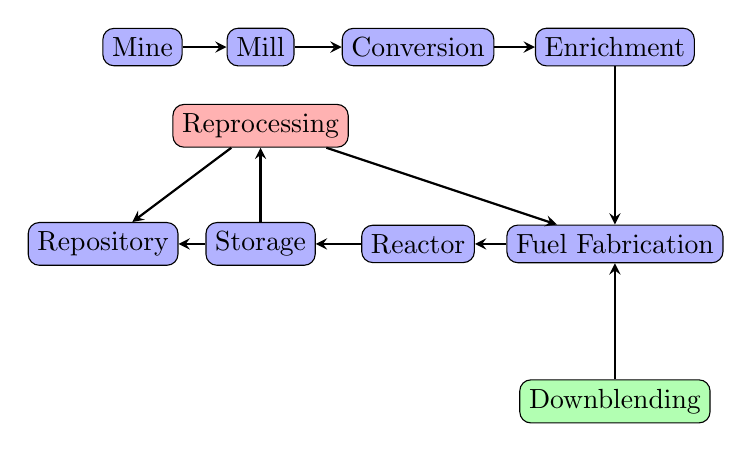
\begin{tikzpicture}[node distance=1cm]
        \node (mine) [agent] {Mine};
        \node (mill) [agent, right of=mine, xshift=0.5cm] {Mill};
        \node (conversion) [agent, right of=mill, xshift=1cm] {Conversion};
        \node (enrichment) [agent, right of=conversion, xshift=1.5cm]{Enrichment};
        \node (fabrication) [agent, below of=enrichment, yshift=-1.5cm]{Fuel Fabrication};
        \node (reactor) [agent, left of=fabrication, xshift=-1.5cm]{Reactor};
        \node (storage) [agent,  left of=reactor, xshift=-1cm]{Storage};
        \node (sinkhlw) [agent, left of=storage, xshift=-1cm]{Repository};


        \draw [arrow] (mine) --  (mill); 
        \draw [arrow] (mill) -- (conversion); 
        \draw [arrow] (conversion) -- (enrichment);
        \draw [arrow] (enrichment) -- (fabrication);
        \draw [arrow] (fabrication) -- (reactor);
        \draw [arrow] (reactor) -- (storage);
        \draw [arrow] (storage) -- (sinkhlw);
        \pause
        \node (reprocessing) [transition, above of=storage, yshift=0.5cm]{Reprocessing};
        
        \draw [arrow] (storage) -- (reprocessing);
        \draw [arrow] (reprocessing) -- (fabrication);
        \draw [arrow] (reprocessing) -- (sinkhlw);
        \pause
        \node (downblending) [region, below of=fabrication, yshift=-1cm]{Downblending};
        \draw [arrow] (downblending) -- (fabrication);

        \end{tikzpicture}
    \caption{Overview of the Nuclear Fuel Cycle.}
    \label{fig:fuel_cycle}
\end{figure}
\end{frame}

\begin{frame}
    \frametitle{Enriching natural uranium to produce HALEU}
    \begin{itemize}
        \item Increase the relative abundance $^{235}$U in the fuel
        \item Enrichment facility designs are based on product 
              mass, product assay, and the \gls{SWU} capacity
    \end{itemize}
    \pause
    \vspace{-0.2cm}
    \begin{columns}
        \column{6cm}
            \begin{figure}[t]
    \centering
    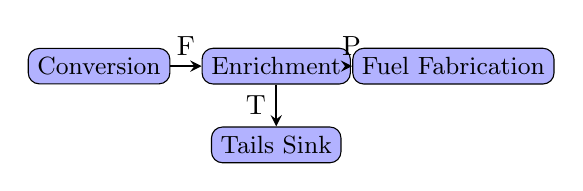
\begin{tikzpicture}[node distance=1cm]
        \node (conversion) [agent] {\small Conversion};
        \node (enrichment) [agent, right of=conversion, xshift=1.25cm]{\small Enrichment};
        \node (fabrication) [agent, right of=enrichment, xshift=1.25cm]{\small Fuel Fabrication};
        \node (sink) [agent, below of=enrichment]{\small Tails Sink};
        
        \draw [arrow] (conversion) -- node[anchor=south]{F} (enrichment);
        \draw [arrow] (enrichment) -- node[anchor=south]{P}(fabrication);
        \draw [arrow] (enrichment) -- node[anchor=east]{T}(sink);

        \end{tikzpicture}
\end{figure}
            \pause
            \begin{align*}
                    & F = P + T \\
                    & x_fF = x_pP + x_tT\\
                    & SWU = \left[P\times V(x_p) +T*V(x_t) - F*V(x_f)\right]*t\\
                    & \text{in which:}\\
                    & V(x_i) = (2x_i - 1)*\ln\left(\frac{x_i}{1-x_i}\right)
            \end{align*}
            \vspace{-0.5cm}
            
    \column{4.5cm}
    \begin{table}
        \centering
        \vspace{-0.3cm}
        \begin{tabular}{c m{2.5cm}}
            \hline
            Variable & Definition \\
            \hline
            F & Feed mass \\
            P & Product mass \\
            T & Tails mass\\
            x$_i$ & Assay of material stream $i$\\
            SWU & Separative work units\\
            V(x$_i$) & Separation potential function\\
            t & Time\\
            \hline
        \end{tabular}
    \end{table}

    \end{columns}
\end{frame}

\begin{frame}
    \frametitle{Downblending HEU to produce HALEU}
    If we downblend \gls{HEU} to produce \gls{HALEU}:
    \begin{itemize}
        \item Spent fuel from \gls{EBR} can produce 10 MT of \gls{HALEU}
              \cite{nuclear_energy_institute_establishing_2022}
        \item \gls{HEU} from \gls{SRS} can produce 4-20 MT of \gls{HALEU}
              \cite{nuclear_energy_institute_establishing_2022,regalbuto_addressing_2020}
        \item<2-> The fuel will have uranium impurities that are not typically 
              in enriched fuel or considered for reactor modeling 
              \cite{nelson_foreign_2010,vaden_isotopic_2018}
    \end{itemize}
\end{frame}

\begin{frame}
    \frametitle{Efforts to estimate HALEU needs}
    Efforts are underway to estimate potential \gls{HALEU} needs:
    \begin{itemize}
        \item \gls{NEI} surveyed multiple reactor design companies
              to estimate \gls{HALEU} needs between now and 2035 
              \cite{korsnick_updated_2021,nuclear_energy_institute_establishing_2022}
        \item National labs modeled the transition to some 
              \gls{HALEU}-fueled reactors to estimate \gls{HALEU} needs 
              to meet current net-zero carbon goals in 2050 \cite{dixon_estimated_2022}
    \end{itemize}
    \pause
    Limitations of this previous work:
    \begin{itemize}
        \item All start from announced advanced reactor projects
        \item Very prescriptive in reactor deployment
        \item<3-> Mostly concerned with \gls{HALEU} mass, don't consider 
              other fuel cycle needs for \gls{HALEU}-fueled reactors
    \end{itemize}
\end{frame}

\subsection{Objectives}
\begin{frame}
    \frametitle{Technical gaps \& objectives}
    \begin{block}{Technical Gaps}
        \begin{itemize}
            \item Understand changes to the US nuclear fuel cycle to 
                  commercially supply \gls{HALEU}
            \item Understand limitations of using downblended \gls{HEU} 
                  in advanced reactors         
        \end{itemize}
    \end{block}
    \pause
    \begin{block}{Objectives}
        \begin{itemize}
        \item<2-> Explore how the deployment of \gls{HALEU}-fueled reactors 
        affects the US nuclear fuel cycle 
        \item<2-> Quantify potential material requirements for the transition from 
              \glspl{LWR} to advanced reactors in a once-through and recycling 
              fuel cycle
        \item<2-> Understand the impacts of fuel cycle parameters on the 
              material requirements and design optimized transition scenarios
        \item<2-> Identify potential limitations in using downblended \gls{HEU} 
              in advanced reactors
        \end{itemize}
    \end{block}
\end{frame}
\section{Transition analysis}
\begin{frame}
    \frametitle{Transition analysis}
    To meet the second objective, I model the transition from the current 
    \gls{LWR} fleet to advanced reactors
    \begin{itemize}
        \item<2-> Use \Cyclus \cite{huff_fundamental_2016}, 
              a fuel cycle simulator, to model the transition
        \item<3-> Model the deployment and decommissioning of fuel cycle facilities 
        \item<3-> Model material transactions between facilities
        \item<4-> Quantify material requirements for different fuel cycles
    \end{itemize}

\end{frame}

\subsection{Once-through fuel cycles}
\begin{frame}
    \frametitle{Transition analysis assumptions}
    \begin{columns}
        
    \column[t]{6cm}
    \vspace{-0.9cm}
    \begin{figure}
    \centering
    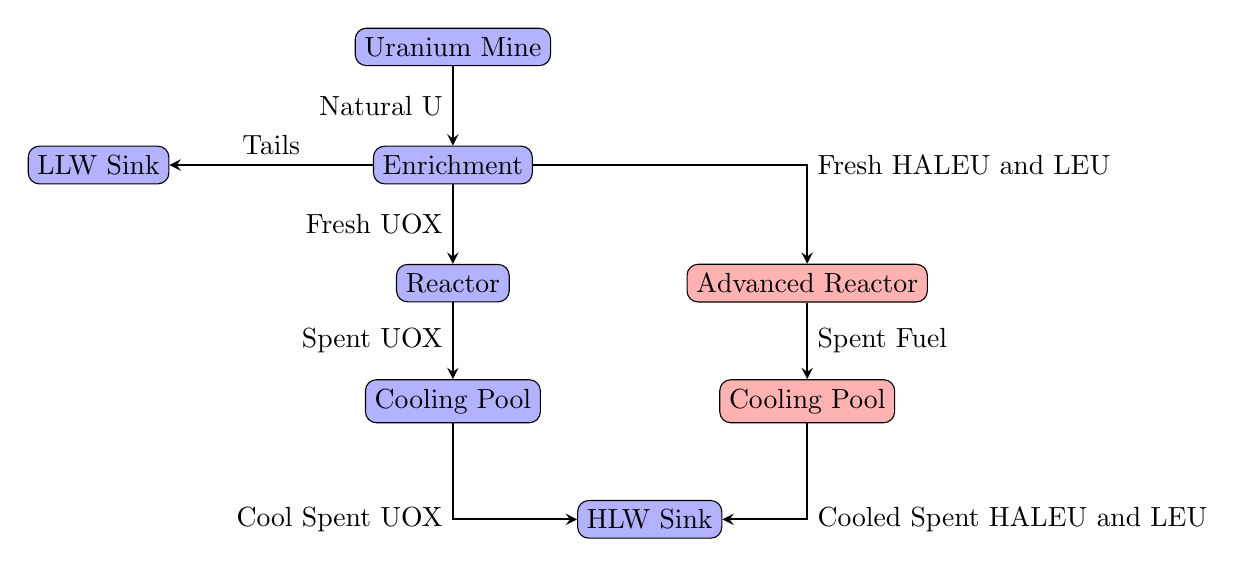
\begin{tikzpicture}[node distance=1.5cm]
        \node (mine) [facility] {Uranium Mine};
        \node (enrichment) [facility, below of=mine]{Enrichment};
        \node (reactor) [facility, below of=enrichment]{Reactor};
        \node (adv_reactor) [transition, right of=reactor, xshift=3cm]{Advanced Reactor};
        \node (wetstorage) [facility, below of=reactor]{Cooling Pool};
        %\node (drystorage) [facility, below of=wetstorage]{Dry Storage};
        \node (cooling) [transition, below of=adv_reactor]{Cooling Pool};
        \node (sinkhlw) [facility, below of=wetstorage, xshift=2.5cm]{HLW Sink};
        \node (sinkllw) [facility, left of=enrichment, xshift=-3cm]{LLW Sink};

        \draw [arrow] (mine) -- node[anchor=east]{Natural U} (enrichment);  
        \draw [arrow] (enrichment) -- node[anchor=south]{Tails}(sinkllw);
        \draw [arrow] (enrichment) -- node[anchor=east]{Fresh UOX}(reactor);
        \draw [arrow] (enrichment) -| node[anchor=west]{Fresh HALEU and LEU}(adv_reactor);
        \draw [arrow] (reactor) -- node[anchor=east]{Spent UOX}(wetstorage);
        \draw [arrow] (wetstorage) |- node[anchor=east]{Cool Spent UOX}(sinkhlw);
        %\draw [arrow] (drystorage) |- node[anchor=east]{Casked Spent UOX}(sinkhlw);
        \draw [arrow] (adv_reactor) -- node[anchor=west]{Spent Fuel}(cooling);
        \draw [arrow] (cooling) |- node[anchor=west]{Cooled Spent HALEU and LEU}(sinkhlw);`'

        \end{tikzpicture}
    \caption{Fuel cycle facilities and material flow between facilities in the 
    once-through fuel cycles modeled. Facilities in 
    blue are used in all once-through scenarios, the facilities in red are added in
    at the transition start time in the transition scenarios.}
    \label{fig:once-through_fuel_cycle}
\end{figure}

        \column[t]{4.5cm}
        \begin{itemize}
            \item Simulations model reactor deployment from 1965-2090
            \item Transitions begin in 2025
            \item<2-> \gls{LWR} commission dates are obtained from the IAEA PRIS
                database \cite{noauthor_power_1989}
            \item<2-> \glspl{LWR} are assumed to operate until their current license 
                expires
            \item<3-> Manually calculate advanced reactor deployment
            \item<3-> Assume natural uranium is enriched to produce all 
                  fuel
        \end{itemize}

\end{columns}
\end{frame}

\begin{frame}
    \frametitle{Advanced reactors}
    \vspace{-0.2cm}
    \begingroup
        \renewcommand{\arraystretch}{1.5}
        \begin{table}
            \small
            \caption{Advanced reactor design specifications}
            \label{tab:reactor_summary}
            \vspace{-0.15cm}
            \begin{tabular}{ l p{1.5cm} p{1.5cm} p{2cm} }
                \hline
                Design Criteria & USNC MMR 
                    \cite{noauthor_usnc_2021} & 
                    X-energy Xe-100 \cite{mulder_overview_2021} & 
                    NuScale VOYGR \cite{nuscale_chapter_2020-1,reyes_nuscale_2021,reyes_correction_2022}\\\hline
                Reactor type & HTGR & HTGR & SMR\\
                Fuel type & UO$_2$ FCM & UCO TRISO & UO$_2$ pellets \\
                Power (MWe) & 5 & 80 & 77\\
                Power (MWth) & 15 & 200 & 250\\
                Enrichment (\% $^{235}U$) & 19.75 & 15.5 & 4.09 \\
                Cycle Length (yr) & 20 & Online & 1.5 \\
                Number of cycles & 1 & 6 & 3\\
                Reactor Lifetime (yr) & 20 & 60 & 60\\
                Burnup ($\frac{MWd}{kg U}$) & 82 & 168 & 45\\
                \hline
            \end{tabular}
        \end{table}   
    \endgroup
    \begin{equation}
        \text{mass (kg)} = \frac{\text{Power (MWth) * cycle length (d)*number of cycles}}{\text{Burnup (MWd/kg)}}
        \label{eq:fuel_mass}
    \end{equation}
\end{frame}

\begin{frame}
    \frametitle{Once-through scenario definitions}
        \begin{table}[ht]
            \centering
            \caption{Summary of the once-through fuel cycle transition scenarios.
                     Energy growth is relative to energy from \glspl{LWR} in 2025.}
            \label{tab:scenarios_once-through}
            \begin{tabular}{c l l}
                    \hline
                    Scenario number & Reactors present & Energy demand\\\hline
                    \rowcolor{lightblue} 1 & \glspl{LWR} & N/A \\
                    \rowcolor{lightorange}2 & \glspl{LWR} and MMR & No growth \\
                    \rowcolor{lightorange}3 & \glspl{LWR} and Xe-100 & No growth \\
                    \rowcolor{lightorange}4 & \glspl{LWR}, Xe-100, and MMR& No growth\\
                    \rowcolor{lightorange}5 & \glspl{LWR}, MMR, and VOYGR & No growth\\
                    \rowcolor{lightorange}6 & \glspl{LWR}, Xe-100, and VOYGR & No growth\\
                    \rowcolor{lightorange}7 & \glspl{LWR}, Xe-100, MMR, and VOYGR & No growth\\
                    \rowcolor{lightpink}8 & \glspl{LWR} and MMR& 1\% growth \\
                    \rowcolor{lightpink}9 & \glspl{LWR} and Xe-100 & 1\% growth\\
                    \rowcolor{lightpink}10 & \glspl{LWR}, Xe-100, and MMR& 1\% growth\\
                    \rowcolor{lightpink}11 & \glspl{LWR}, MMR, and VOYGR & 1\% growth\\
                    \rowcolor{lightpink}12 & \glspl{LWR}, Xe-100, and VOYGR & 1\% growth\\
                    \rowcolor{lightpink}13 & \glspl{LWR}, Xe-100, MMR, and VOYGR & 1\% growth\\
                    \hline
            \end{tabular}
        \end{table}
        %<2-> \tikz[overlay, remember picture]{\draw{draw=red,thick, double, fillopacity=0.2] ($(infrastructure)+(-0.5,0.4)$) rectangle ($(infrastructure)+(6,-0.2)$);}} 
\end{frame}

\begin{frame}
    \frametitle{Once-through scenario definitions}
        \begin{table}[ht]
            \centering
            \caption{Summary of the once-through fuel cycle transition scenarios.
            Energy growth is relative to energy from \glspl{LWR} in 2025.}
            \label{tab:scenarios_once-through}
            \begin{tabular}{c l l}
                \hline
                Scenario number & Reactors present & Energy demand\\\hline
                \rowcolor{lightblue} 1 & \glspl{LWR} & N/A \\
                \rowcolor{lightorange}\marktopleft{a3}2 & \glspl{LWR} and MMR & No growth \\
                \rowcolor{lightorange}3 & \glspl{LWR} and Xe-100 & No growth \\
                \rowcolor{lightorange}4 & \glspl{LWR}, Xe-100, and MMR& No growth\\
                \rowcolor{lightorange}5 & \glspl{LWR}, MMR, and VOYGR & No growth\\
                \rowcolor{lightorange}6 & \glspl{LWR}, Xe-100, and VOYGR & No growth\\
                \rowcolor{lightorange}7 & \glspl{LWR}, Xe-100, MMR, and VOYGR & No growth
                \markbottomright{a3}\\
                \rowcolor{lightpink}8 & \glspl{LWR} and MMR& 1\% growth \\
                \rowcolor{lightpink}9 & \glspl{LWR} and Xe-100 & 1\% growth\\
                \rowcolor{lightpink}10 & \glspl{LWR}, Xe-100, and MMR& 1\% growth\\
                \rowcolor{lightpink}11 & \glspl{LWR}, MMR, and VOYGR & 1\% growth\\
                \rowcolor{lightpink}12 & \glspl{LWR}, Xe-100, and VOYGR & 1\% growth\\
                \rowcolor{lightpink}13 & \glspl{LWR}, Xe-100, MMR, and VOYGR & 1\% growth\\
                \hline
        \end{tabular}
        \end{table}
        %<2-> \tikz[overlay, remember picture]{\draw{draw=red,thick, double, fillopacity=0.2] ($(infrastructure)+(-0.5,0.4)$) rectangle ($(infrastructure)+(6,-0.2)$);}} 
\end{frame}

\begin{frame}
    \frametitle{Advanced reactor deployment scheme}
    \begin{columns}
        \column[t]{5cm}
            Manually calculate the deployment scheme for advanced reactors
            \begin{itemize}
                \item Preferentially deploy reactors with larger power output first
                \item Deploy reactor with largest power output until an oversupply 
                      of power would be produced, deploy the next reactor until 
                      an oversupply of power, then deploy the last reactor until 
                      demand is met
                \item Deployment schedule is given to \Cyclus
            \end{itemize}
        \column[t]{5.5cm}
            \begin{figure}
                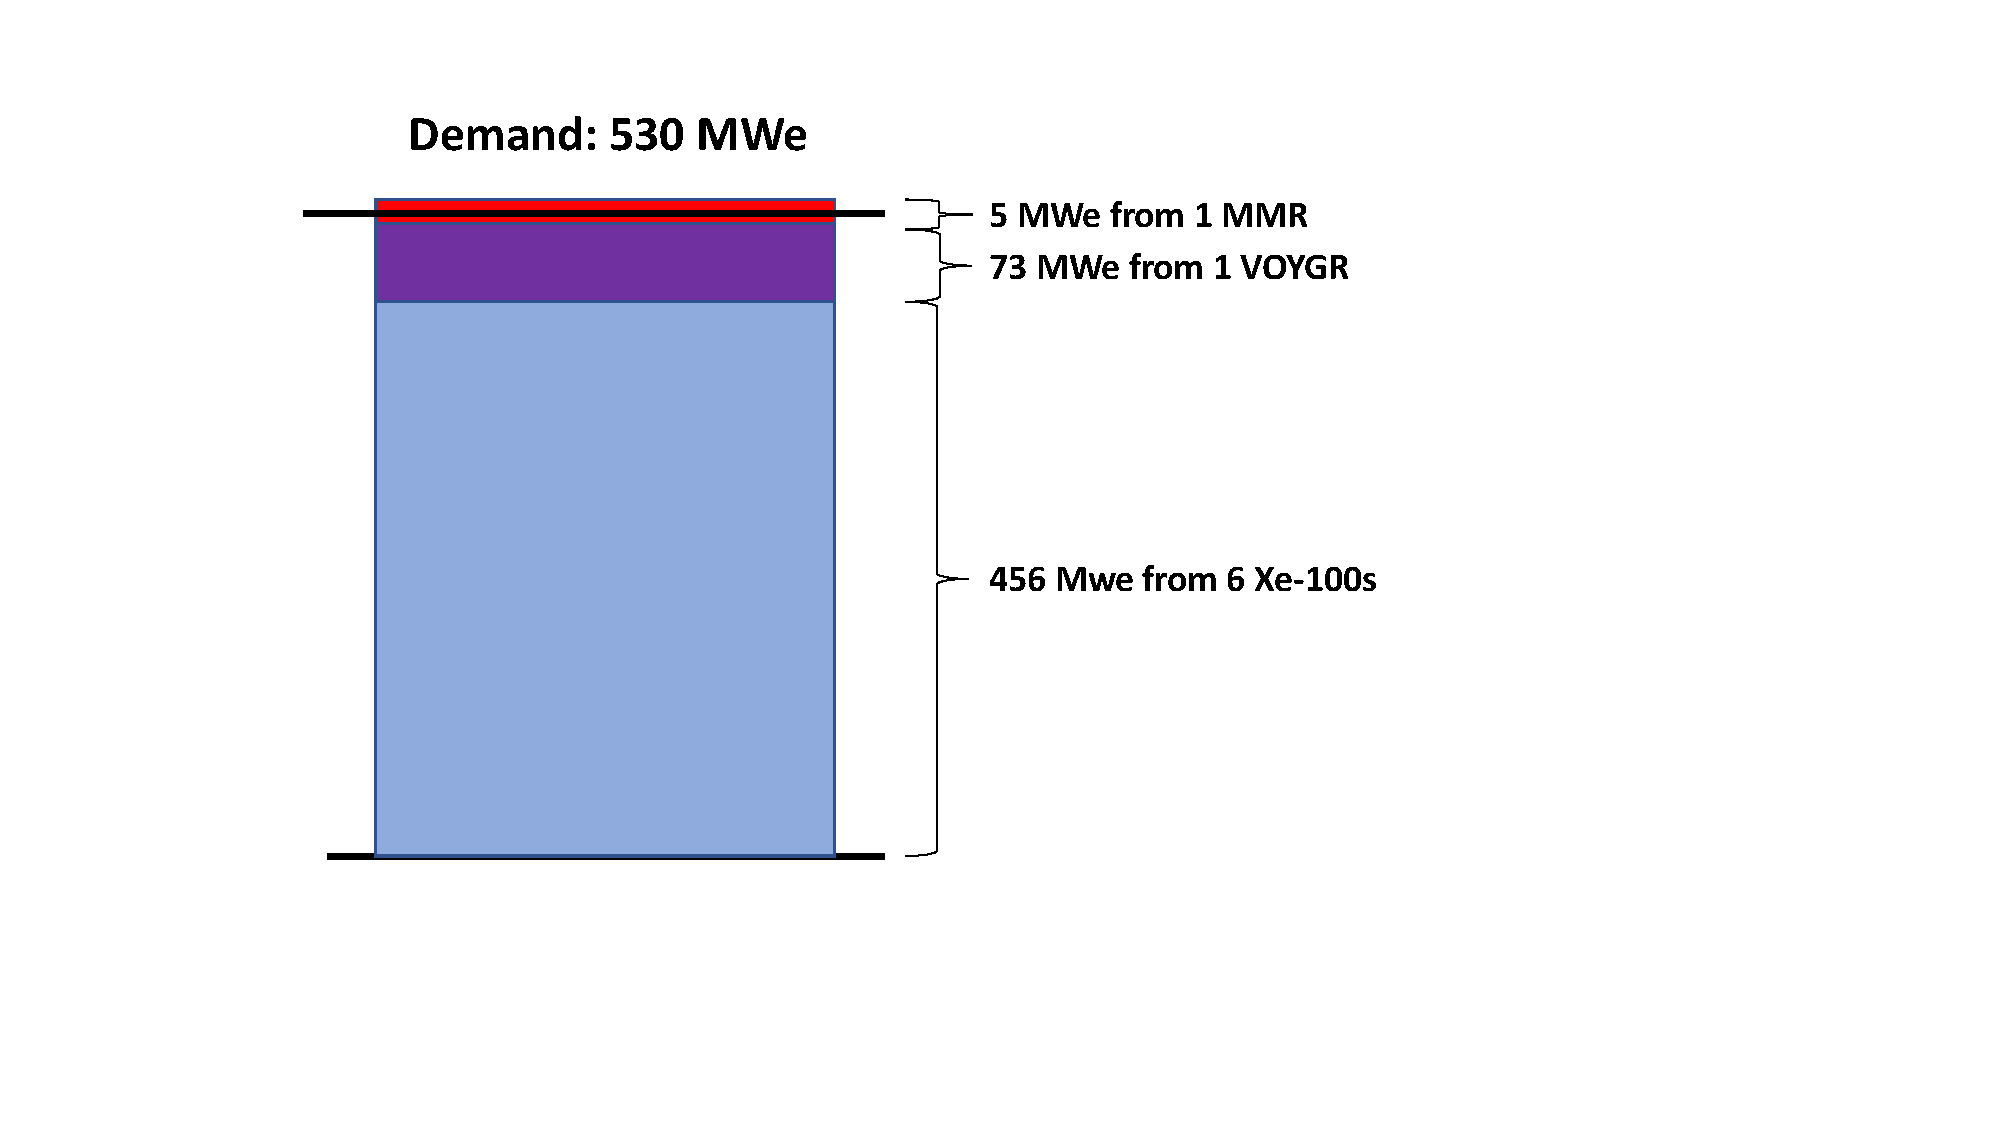
\includegraphics[scale=0.3, trim=150 100 50 50,clip]{Deployment_Scheme.pdf}
                \caption{Example of how advanced reactors in Scenario 7 are deployed to 
                meet a fictitious demand of 530 MWe.}
                \label{fig:deployment}
            \end{figure}
                    
    \end{columns}
\end{frame}
\subsection{Once-through results}

\begin{frame}
    \frametitle{Number of reactors}
    %\begin{columns}
        %\column[t]{4.3cm}
            \begin{itemize}
                \item Number of reactors deployed scales with the power 
                      output of each reactor type
                \item Scenario 2 (MMR) deploys the most reactors
                \item Scenario 3 (Xe-100) deploys the fewest reactors
                \item Similar number of Xe-100s and VOYGRs are deployed
                \item Scenarios 4 (Xe-100+MMR), 6 (Xe-100+VOYGR), and 7 
                      (Xe-100+VOYGR+MMR) mostly deploy Xe-100s 
                \item Scenario 5 (MMR+VOYGR) mostly deploys VOYGRs
            \end{itemize}
        %\column[t]{5.7cm}
        %\vspace{-0.5cm}
        \begin{figure}
        \begin{subfigure}{0.48\textwidth}
                \centering
                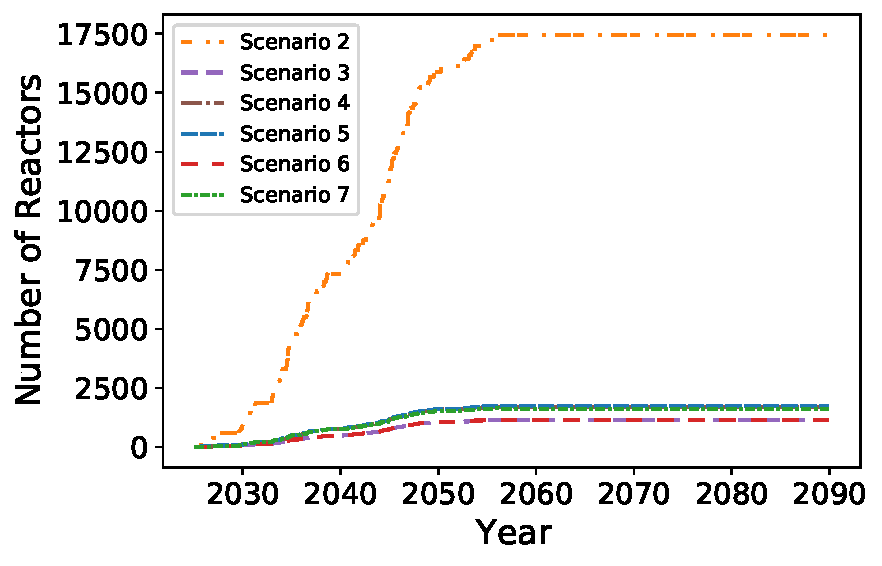
\includegraphics[width=\textwidth]{nogrowth_reactors.pdf}
        \end{subfigure}
        \hfill
        \begin{subfigure}{0.48\textwidth}
            \centering
            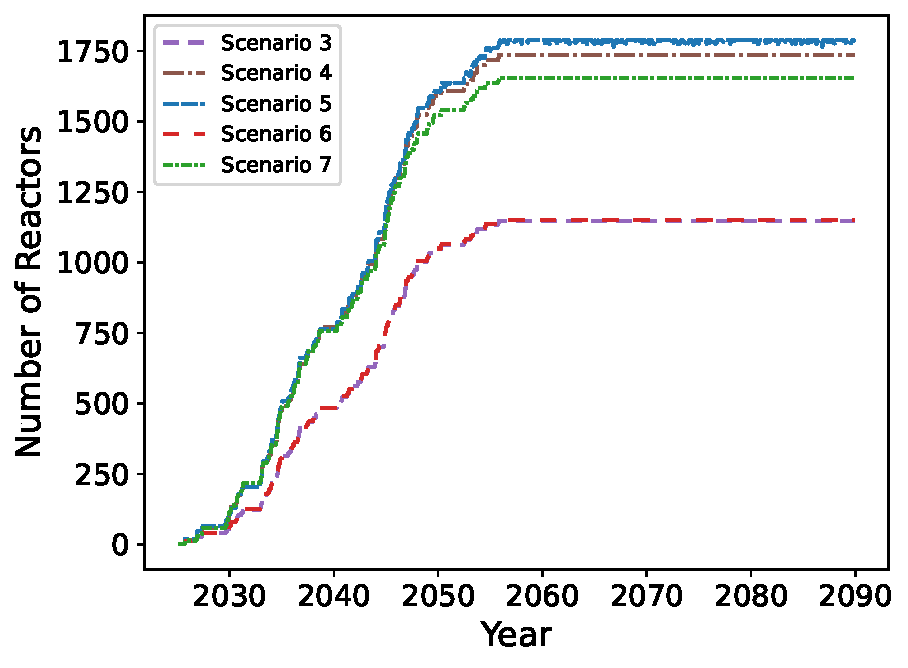
\includegraphics[width=\textwidth]{nogrowth_reactors_3-7.pdf}
        \end{subfigure}
        \vspace{-0.15cm}
        \caption{Number of advanced reactors deployed in Scenarios 2-7 (left)
        and Scenarios 3-7 (right).}
        \end{figure}
    %\end{columns}
\end{frame}

\begin{frame}
    \frametitle{Reactor designs drives the uranium mass required}
    \begin{columns}
        \column[t]{4.5cm}
            \begin{itemize}
                \item Scenario 5 (MMR + VOYGR) requires the largest average mass of 
                      enriched uranium
                \item Scenario 2 (MMR) requires the largest mass of \gls{HALEU}
                \item Scenario 3 (Xe-100) requires the smallest mass of enriched 
                      uranium
                \item Scenario 5 (MMR + VOYGR) requires the smallest mass of \gls{HALEU}
            \end{itemize}
        \column[t]{5.5cm}
        \vspace{-0.8cm}
            \begin{figure}
                \centering
                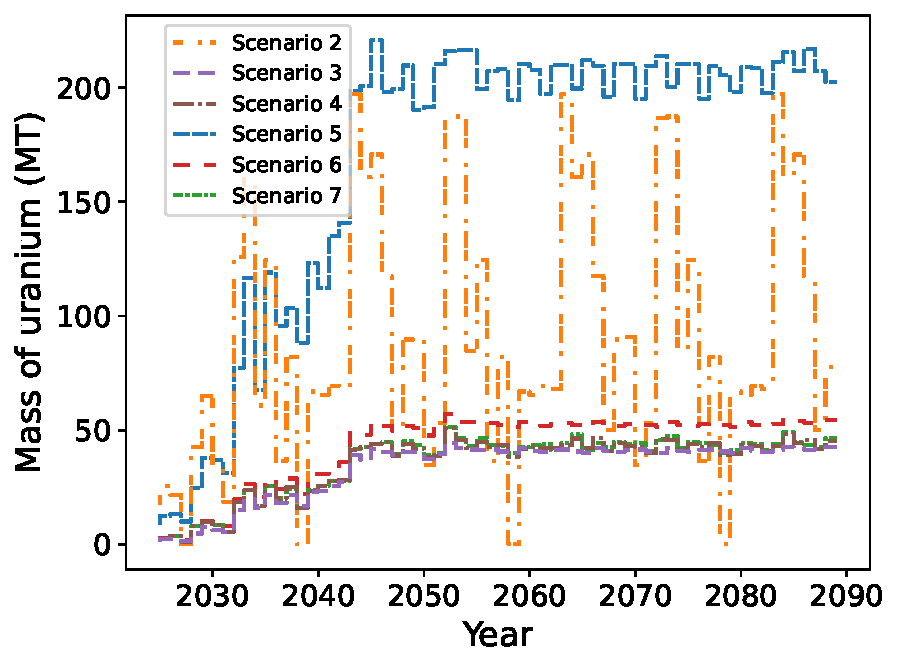
\includegraphics[scale=0.43]{nogrowth_AR_uranium.pdf}
                \caption{Annual average mass of enriched uranium required to fuel
                advanced reactors in Scenarios 2-7.}
                \label{fig:uranium}

        \end{figure}
    \end{columns}
\end{frame}

\begin{frame}
    \frametitle{Advanced reactor designs}
    \begingroup
        \renewcommand{\arraystretch}{1.5}
        \begin{table}
            \small
            \caption{Advanced reactor design specifications}
            \label{tab:reactor_summary}
            \begin{tabular}{ c c c c }
                \hline
                Design Criteria & MMR 
                    \cite{noauthor_usnc_2021} & 
                    Xe-100 \cite{mulder_overview_2021} & 
                    VOYGR \cite{nuscale_chapter_2020-1,reyes_nuscale_2021,reyes_correction_2022}\\\hline
                Power (MWe) & 5 & 80 & 77\\
                Power (MWth) & 15 & 200 & 250\\
                Enrichment (\% $^{235}U$) & 19.75 & 15.5 & 4.09 \\
                Cycle Length (yr) & 20 & Online & 1.5 \\
                Number of cycles & 1 & 6 & 3\\
                Reactor Lifetime (yr) & 20 & 60 & 60\\
                Burnup ($\frac{MWd}{kg U}$) & 82 & 168 & 45\\
                \hline
            \end{tabular}
        \end{table}   
    \endgroup
    \begin{equation*}
        \text{mass (kg)} = \frac{\text{Power (MWth) * cycle length (d)*number of cycles}}{\text{Burnup (MWd/kg)}}
        \label{eq:fuel_mass}
    \end{equation*}
\end{frame}

\begin{frame}
    \frametitle{\gls{SWU} capacity is a function of product mass and assay}
    \begin{columns}
        \column[t]{4.3cm}
            \begin{itemize}
                \item Follows similar pattern to feed uranium  mass 
                \item Scenario 2 (MMR) requires the largest average \gls{SWU} 
                \item The other scenarios are comparable for the average 
                      capacity they require
                \item \gls{SWU} capacity is a function of product mass and 
                      product assay
                
            \end{itemize}
        \column[t]{5.7cm}
        \vspace{-1cm}
        \begin{figure}
                \centering
                \includegraphics[scale=0.43]{nogrowth_AR_swu.pdf}
                \caption{Annual average \gls{SWU} capacity required to produce 
                enriched uranium for and advanced reactors in Scenarios 2-7.}
                \label{fig:swu}
        \end{figure}
    \end{columns}
\end{frame}

\begin{frame}
    \frametitle{\gls{SNF} discharged follows with fuel mass}
    \begin{columns}
        \column[t]{4.3cm}
            \begin{itemize}
                \item Scenario 5 (MMR + VOYGR) discharges the largest mass of \gls{SNF}
                \item Scenario 3 (Xe-100) discharges the least \gls{SNF}
                \item Scenario 2 (MMR) discharges \gls{SNF} the latest
                \item Cumulative masses range between 25,654 MT (Scenario 3) to 
                      112,913 MT (Scenario 5)
                
            \end{itemize}
        \column[t]{5.7cm}
        \vspace{-1cm}
        \begin{figure}
                \centering
                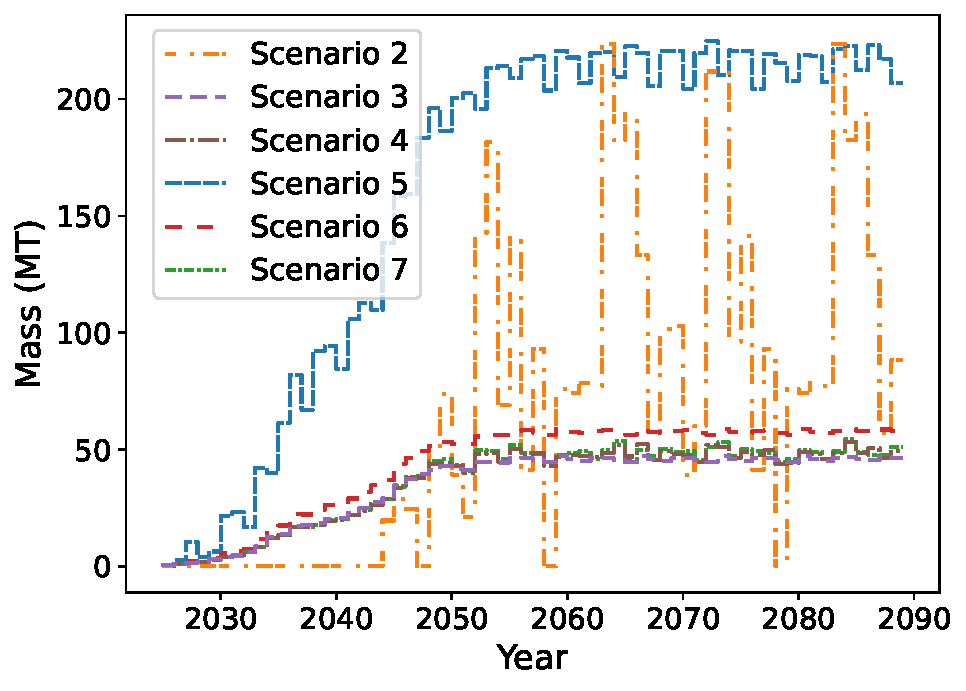
\includegraphics[scale=0.43]{nogrowth_AR_waste.pdf}
                \caption{Annual average mass of \gls{SNF} discharged from 
                advanced reactors in Scenarios 2-7.}
                \label{fig:waste}
        \end{figure}
    \end{columns}
\end{frame}
\subsection{Closed fuel cycles}
\begin{frame}
    \frametitle{What about a different fuel cycle option?}
    What if we had a closed fuel cycle that required \gls{HALEU}?
    \begin{itemize}
        \item How does the fuel cycle option impact the material requirements?
        \item Does this save resources?
    \end{itemize}

\end{frame}

\begin{frame}
    \frametitle{Recycling needs accurate spent fuel compositions}
    \begin{itemize}
    \item \Gls{SNF} compositions impact numerous fuel cycle considerations:
    \begin{itemize}
        \item decay heat
        \item criticality safety
        \item amount of plutonium and transuranic elements
    \end{itemize}
    \item<2-> \Cyclus uses archetypes to model reactors, and the physics 
         of a reactor
    \item<2-> Different reactor archetypes use different methodologies 
         to model fuel depletion
    \item<3-> The \Cycamore \texttt{Reactor} uses recipes to define spent fuel compositions
    \item<3-> Other \Cyclus reactor archetypes can dynamically model 
          fuel depletion, but they require export controlled software 
          or are reactor design specific
\end{itemize}
\end{frame}

\begin{frame}
    \frametitle{OpenMCyclus: an open source coupling with OpenMC}
    \begin{columns}
        \column[t]{5cm}
    \begin{itemize}
        \item Developed a reactor archetype that couples \Cyclus with 
              stand-alone depletion solver in OpenMC
        \item Publicly available on GitHub \cite{bachmann_openmcyclus_2023}
        \item<2-> Compared against the \Cycamore \texttt{Reactor} in a 
              simple closed fuel cycle
    \end{itemize}

    \column[t]{6.5cm}\begin{figure}[h!]
        \centering
        \small
        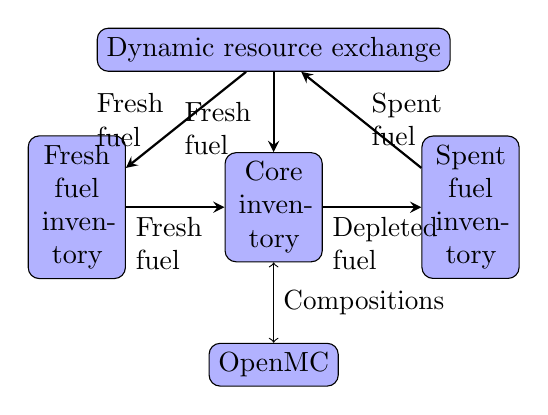
\begin{tikzpicture}[node distance=2cm]
            \node (dre) [facility] {Dynamic resource exchange};
            \node (fresh) [facility, below of=dre, xshift=-2.5cm,text width=1cm]{Fresh fuel inventory};
            \node (core) [facility, below of=dre, text width=1cm]{Core inventory};
            \node (spent) [facility, below of=dre, xshift=2.5cm,text width=1cm]{Spent fuel inventory};
            \node (openmc) [facility, below of=core]{OpenMC};

            \draw [arrow] (dre) -- node[anchor=east, text width=1cm]{Fresh fuel} (fresh);
            \draw [arrow] (dre) -- node[anchor=east, text width=1cm,pos=0.7]{Fresh fuel} (core);
            \draw [arrow] (fresh) -- node[anchor=north, text width=1cm]{Fresh fuel} (core);
            \draw [arrow] (core) -- node[anchor=north, text width=1cm]{Depleted fuel} (spent);
            \draw [arrow] (spent) -- node[anchor=west, text width=1cm]{Spent fuel} (dre);
            \draw [<->] (core) -- node[anchor=west, text width=1cm]{Compositions} (openmc);
            \end{tikzpicture}
        \caption{Material handling pathways between different material 
        inventories in OpenMCyclus and the \gls{DRE} of \Cyclus. }
        \label{fig:openmcyclus-flow}
    \end{figure}

    \end{columns}
\end{frame}

\begin{frame}
    \frametitle{Benchmark description}
    \begin{columns}
        \column[t]{4.5cm}
        \begin{itemize}
            \item Closed fuel cycle with 1 reactor type, modeled with 
                  either \Cycamore or OpenMCyclus
            \item Reactors prefer MOX over UOX
            \item Reactors deployed at time steps 1, 50, 100, 150, with a 
                  60 time step lifetime
            \item<2-> Ran with \Cycamore \texttt{Reactor} twice, toggling 
                  the \texttt{decom\_transmute\_all} setting
            \item<3-> Used OpenMC to get spent fuel compositions and cross section data
        \end{itemize}
        \column[t]{6.3cm}
        \begin{figure}
            \centering
            \small
            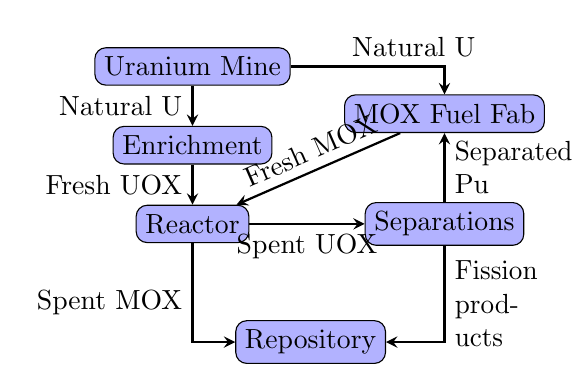
\begin{tikzpicture}[node distance=1cm]
                \node (mine) [facility] {Uranium Mine};
                \node (enrichment) [facility, below of=mine]{Enrichment};
                \node (reactor) [facility, below of=enrichment]{Reactor};
                \node (sinkhlw) [facility, below of=reactor, xshift=1.5cm, yshift=-0.5cm]{Repository};
                \node (separation) [facility, right of=reactor, xshift=2.2cm]{Separations};
                \node (mox_fab) [facility, above of=separation, yshift=0.4cm]{MOX Fuel Fab};
                
                \draw [arrow] (mine) -- node[anchor=east]{Natural U} (enrichment);
                \draw [arrow] (enrichment) -- node[anchor=east]{Fresh UOX}(reactor);
                \draw [arrow] (reactor) -- node[anchor=north]{Spent UOX}(separation);
                \draw [arrow] (separation) -- node[anchor=west, text width=0.5cm]{Separated Pu}(mox_fab);
                \draw [arrow] (separation) |- node[anchor=west, text width=0.5cm, pos=0.3]{Fission products}(sinkhlw);
                \draw [arrow] (mine) -| node[anchor=south, pos=0.4]{Natural U} (mox_fab);
                \draw [arrow] (reactor) |- node[anchor=east, pos=0.3]{Spent MOX} (sinkhlw);
                \draw [arrow] (mox_fab) -- node[anchor=south, sloped]{Fresh MOX} (reactor);
                \end{tikzpicture}
            \caption{Fuel cycle facilities and material flow between facilities for the 
            sample fuel cycle scenarios used to compare the results of the \Cycamore Reactor 
            and OpenMCyclus DepleteReactor archetypes. }
            \label{fig:comparison}
        \end{figure}
    \end{columns}
\end{frame}

\begin{frame}
    \frametitle{Benchmark Results (I)}
    \begin{columns}
        \column[t]{3.5cm}
        \begin{itemize}
            \item Separated plutonium masses differ because of 
                  different depletion methodologies
            \begin{itemize}
                \item<2-> \Cycamore \texttt{Reactor} applies the same 
                          SNF composition
                \item<2-> OpenMCyclus depletes fuel on a per cycle basis
            \end{itemize}
        \end{itemize}
        \column[t]{6.5cm}
        \begin{figure}
            \centering 
            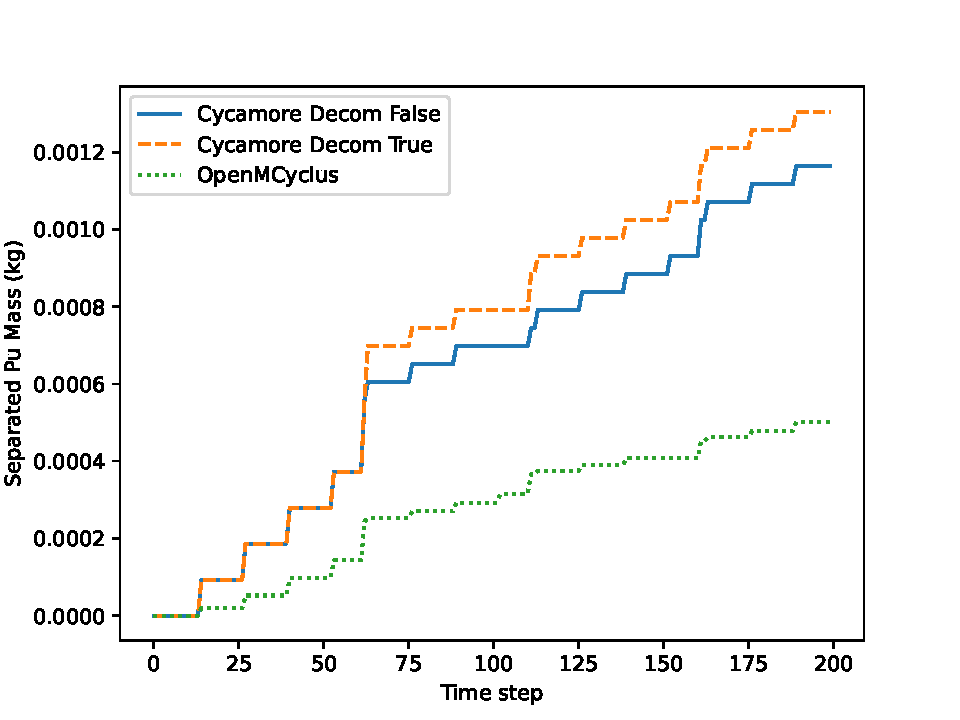
\includegraphics[scale=0.45, trim=0 0 0 30,clip]{comparison_pu_cumulative.pdf}
            \caption{Comparison of cumulative separated plutonium in benchmark between 
            OpenMCyclus and \Cycamore \texttt{Reactor}.}
        \end{figure}
    \end{columns}
\end{frame}

\begin{frame}
    \frametitle{Benchmark Results (I)}
    \begin{columns}
        \column[t]{3.5cm}
        \begin{itemize}
            \item Separated plutonium masses differ because of 
                  different depletion methodologies
                  \begin{itemize}
                    \item \Cycamore \texttt{Reactor} applies the same 
                          SNF composition
                    \item OpenMCyclus depletes fuel on a per cycle basis
                  \end{itemize}
            \item Temporarily changing OpenMCyclus method to better 
                  match with \Cycamore shows better agreement
        \end{itemize}
        \column[t]{6.5cm}
        \begin{figure}
            \centering 
            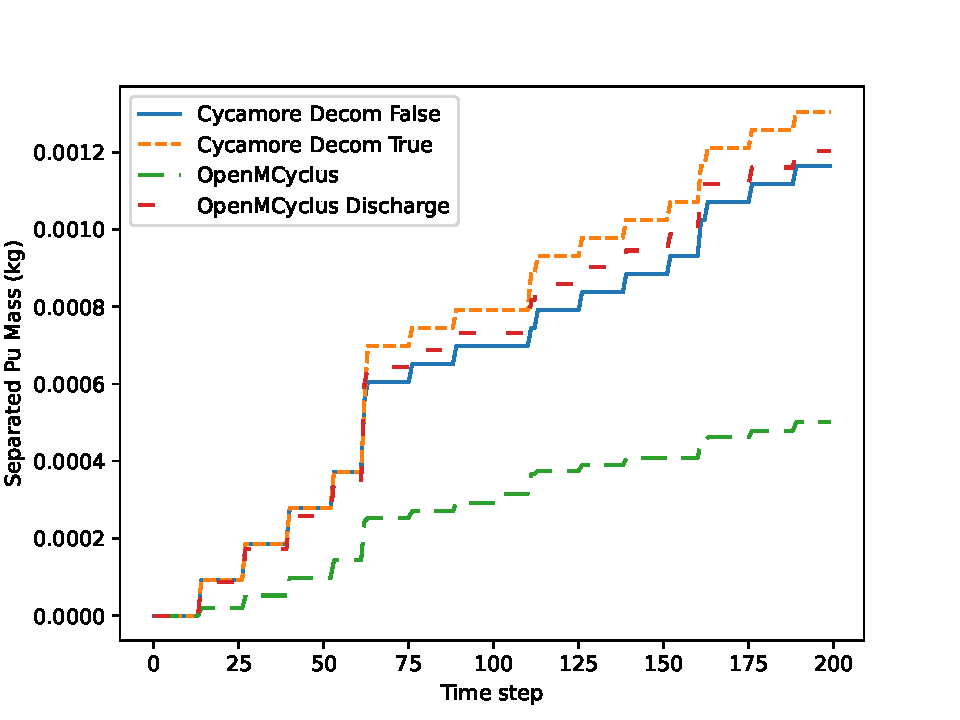
\includegraphics[scale=0.45, trim=0 0 0 30,clip]{comparison_pu_cumulative_discharge.pdf}
            \caption{Comparison of cumulative separated plutonium in benchmark between 
            OpenMCyclus and \Cycamore \texttt{Reactor}.}
        \end{figure}
    \end{columns}
\end{frame}

\begin{frame}
    \frametitle{Benchmark Results (II)}
        \begin{itemize}
            \item Differences in separated plutonium masses 
                  propagate into different fuel receipts 
            \item Spent fuel masses are mostly consistent, except 
                  when a reactor is decommissioned
        \end{itemize}
        \begin{figure}
            \centering
            \begin{subfigure}{0.48\textwidth}
                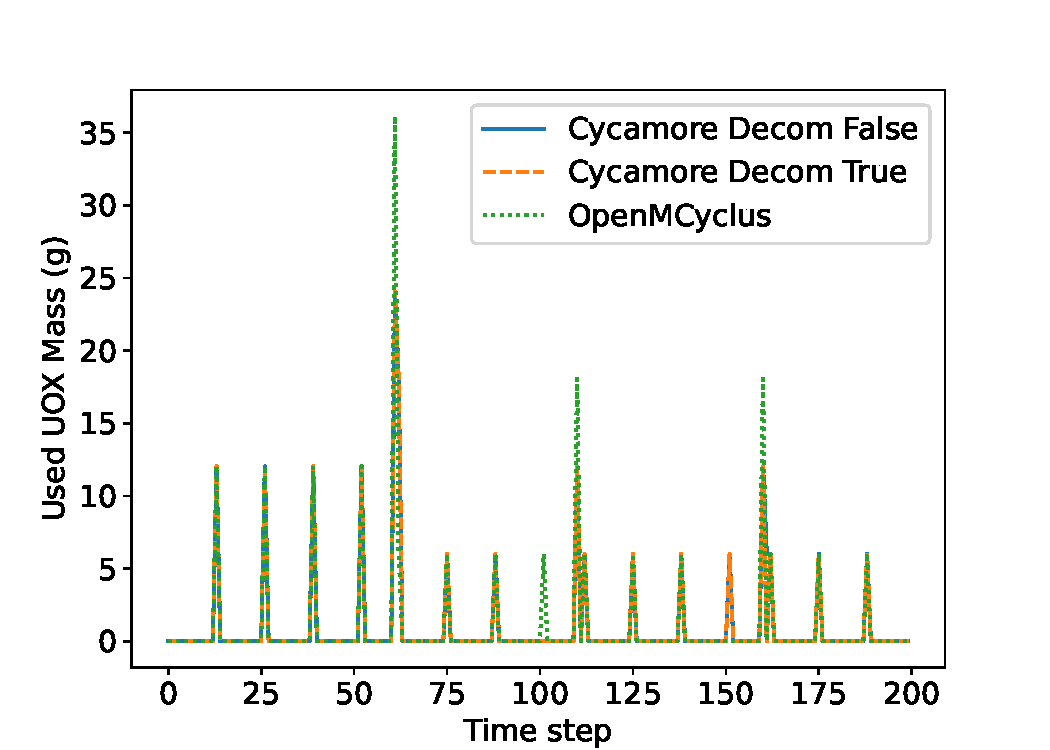
\includegraphics[width=\linewidth]{comparison_spentuox.pdf}
                \caption{Comparison of Spent UOX fuel discharged.}
            \end{subfigure}
            \hfill
            \begin{subfigure}{0.48\textwidth}
                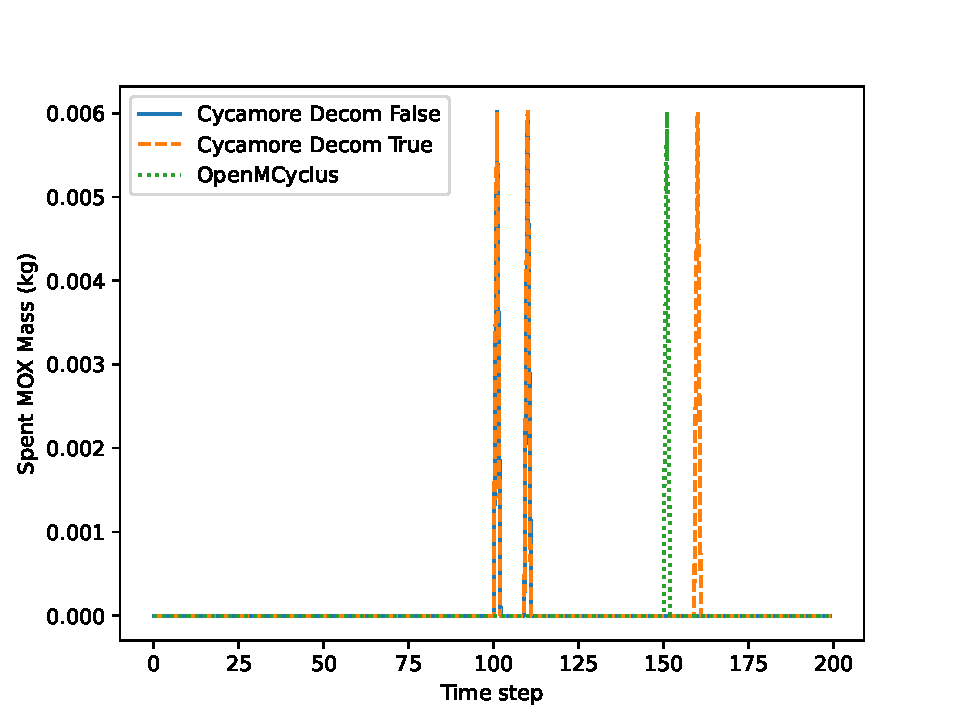
\includegraphics[width=\linewidth]{comparison_spentmox.pdf}
                \caption{Comparison of Spent MOX fuel discharged.}
            \end{subfigure}
            \caption{Spent fuel transactions in OpenMCyclus/\Cycamore benchmark}
            \label{fig:spentfuel_benchmark}
        \end{figure}

\end{frame}

\begin{frame}
    \frametitle{Recycle scenario definitions}
    \begin{table}[ht]
        \centering
        \caption{Summary of the recycle fuel cycle transition scenarios.
        Energy growth is relative to energy from \glspl{LWR} in 2025.}
        \label{tab:scenarios_recycle}
        \begin{tabular}{c l l l}
            \hline
            Scenario & Advanced Reactors & Energy demand & Recycle scheme\\\hline
            \rowcolor{lightorange}14 & Xe-100, MMR, VOYGR & No growth & Limited \\
            \rowcolor{lightorange}15 & Xe-100, MMR, VOYGR & No growth & Limited, no TRISO\\
            \rowcolor{lightorange}16 & SFR& No growth & Continuous \\
            \rowcolor{lightpink}17 & Xe-100, MMR, VOYGR & 1\% growth & Limited \\
            \rowcolor{lightpink}18 & Xe-100, MMR, VOYGR & 1\% growth & Limited, no TRISO\\
            \rowcolor{lightpink}19 & SFR & 1\% growth & Continuous\\
            \hline
    \end{tabular}
    \end{table}
        %<2-> \tikz[overlay, remember picture]{\draw{draw=red,thick, double, fillopacity=0.2] ($(infrastructure)+(-0.5,0.4)$) rectangle ($(infrastructure)+(6,-0.2)$);}} 
\end{frame}

\begin{frame}
    \frametitle{Recycle scenario definitions}
        \begin{table}[ht]
            \centering
            \caption{Summary of the recycle fuel cycle transition scenarios.
            Energy growth is relative to energy from \glspl{LWR} in 2025.}
            \label{tab:scenarios_recycle}
            \begin{tabular}{c l l l}
                \hline
                Scenario & Advanced Reactors & Energy demand & Recycle scheme\\\hline
                \rowcolor{lightorange}\marktopleft{a3}14 & Xe-100, MMR, VOYGR & No growth & Limited \\
                \rowcolor{lightorange}15 & Xe-100, MMR, VOYGR & No growth & Limited, no TRISO\\
                \rowcolor{lightorange}16 & SFR& No growth & Continuous~~~~~~~~\markbottomright{a3}\\
                \rowcolor{lightpink}17 & Xe-100, MMR, VOYGR& 1\% growth & Limited \\
                \rowcolor{lightpink}18 & Xe-100, MMR, VOYGR & 1\% growth & Limited, no TRISO\\
                \rowcolor{lightpink}19 & SFR & 1\% growth & Continuous\\
                \hline
        \end{tabular}
        \end{table}
\end{frame}




\begin{frame}
    \frametitle{Limited recycle fuel cycle assumptions}
    \begin{columns}
        
    \column[t]{6cm}
    \vspace{-0.6cm}
    \begin{figure}
    \centering
    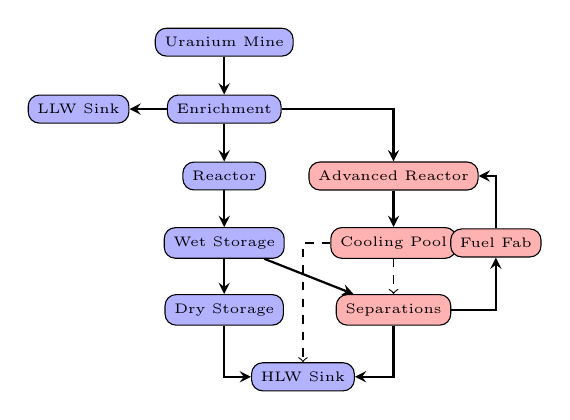
\begin{tikzpicture}[node distance=0.85cm]
        \node (mine) [facility] {\tiny Uranium Mine};
        \node (enrichment) [facility, below of=mine]{\tiny Enrichment};
        \node (reactor) [facility, below of=enrichment]{\tiny Reactor};
        \node (adv_reactor) [transition, right of=reactor, xshift=1.3cm]{\tiny Advanced Reactor};
        \node (wetstorage) [facility, below of=reactor]{\tiny Wet Storage};
        \node (drystorage) [facility, below of=wetstorage]{\tiny Dry Storage};
        \node (cooling) [transition, below of=adv_reactor]{\tiny Cooling Pool};
        \node (sinkhlw) [facility, below of=drystorage, xshift=1cm]{\tiny HLW Sink};
        \node (sinkllw) [facility, left of=enrichment, xshift=-1cm]{\tiny LLW Sink};
        \node (separation) [transition, below of=cooling]{\tiny Separations};
        \node (fuelfab) [transition, below of=adv_reactor,xshift=1.3cm]{\tiny Fuel Fab};
        
        \draw [arrow] (mine) --(enrichment);
        \draw [arrow] (enrichment) -- (reactor);
        \draw [arrow] (enrichment) -- (sinkllw);
        \draw [arrow] (enrichment) -| (adv_reactor);
        \draw [arrow] (reactor) -- (wetstorage);
        \draw [arrow] (wetstorage) -- (drystorage);
        \draw [arrow] (drystorage) |- (sinkhlw);
        \draw [arrow] (adv_reactor) -- (cooling);
        \draw [dashed, ->] (cooling) -- (separation);
        \draw [arrow] (separation) -| (fuelfab);
        \draw [arrow] (fuelfab) |- (adv_reactor);
        \draw [arrow] (separation) |- (sinkhlw);
        \draw [arrow] (wetstorage) -- (separation);
        \draw [dashed, ->] (cooling) -| (sinkhlw);

        \end{tikzpicture}
    \caption{Fuel cycle facilities and material flow between facilities for the recycling 
    scenarios.}
    \label{fig:limited_fuel_cycle}
\end{figure}

        \column[t]{4.5cm}
        \vspace{-0.5cm}
        \begin{itemize}
            \item Reprocess uranium-based fuel, dispose plutonium-based fuel
            \item Reactors prefer plutonium-based fuel over uranium-based fuel
            \item Separations remove only plutonium (aqueous reprocessing)
            \item<2-> Use the same deployment schedule as Scenarios 7, 13
            \item<2-> Modeled Xe-100 and VOYGR with OpenMCyclus
            \item<3-> Separations start in 2020
            \item<3-> Vary if \gls{TRISO} \gls{SNF} is reprocessed
        \end{itemize}

\end{columns}
\end{frame}

\begin{frame}
    \frametitle{Continuous recycle fuel cycle assumptions}
    \begin{columns}
        
    \column[t]{6cm}
    \vspace{-0.5cm}
    \begin{figure}
    \centering
    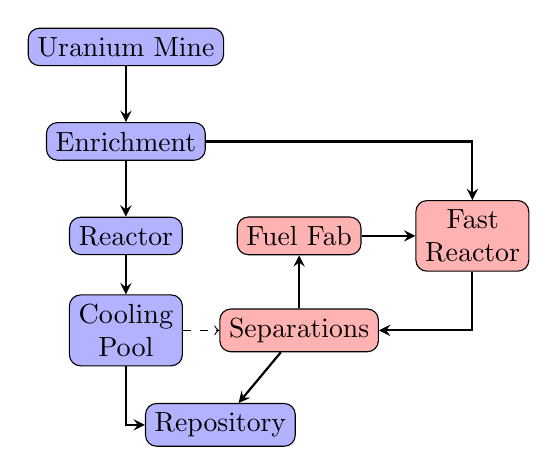
\begin{tikzpicture}[node distance=1.2cm]
        \node (mine) [facility] {Uranium Mine};
        \node (enrichment) [facility, below of=mine]{Enrichment};
        \node (reactor) [facility, below of=enrichment]{Reactor};
        \node (wetstorage) [facility, below of=reactor, text width=1.2cm]{Cooling Pool};
        \node (sinkhlw) [facility, below of=wetstorage, xshift=1.2cm]{Repository};
        \node (separation) [transition, right of=wetstorage,xshift=1cm]{Separations};
        \node (fuelfab) [transition, above of=separation]{Fuel Fab};
        %\node (fr_enrichment) [transition, right of=enrichment,xshift=3cm, text width=1.2cm]{FR Enrichment};
        \node (sfr) [transition, right of=fuelfab, xshift=1.cm,text width=1.2cm]{Fast Reactor};
        
        \draw [arrow] (mine) -- (enrichment);
        \draw [arrow] (enrichment) -- (reactor);
        \draw [arrow] (reactor) -- (wetstorage);
        \draw [arrow] (wetstorage) |- (sinkhlw);
        \draw [arrow] (separation) -- (fuelfab);
        \draw [arrow] (separation) -- (sinkhlw);
        \draw [arrow] (fuelfab) -- (sfr);
        \draw [dashed, ->] (wetstorage) -- (separation);
        \draw [arrow] (sfr) |- (separation);
        \draw [arrow] (enrichment) -| (sfr);

        \end{tikzpicture}
    \caption{Fuel cycle facilities and material flow between facilities for 
    the continuous recycling scenarios.}
    \label{fig:continuous_fuel_cycle}
\end{figure}

        \column[t]{4.5cm}
        \begin{itemize}
            \item Reprocess all \gls{SNF} 
            \item Introduce a fast reactor for transition, modeled through 
                  OpenMCyclus
            \item Separation start 2020
            \item Can accept plutonium-based fuel (preferred) or \gls{HALEU}
            \item Separations remove U, Np, Pu, Am (electrochemical reprocessing)
            \item<2-> Use the same deployment scheme for the fast reactor
            \item<3-> Assume natural uranium is enriched to produce 
                  fuel
        \end{itemize}

\end{columns}
\end{frame}

\begin{frame}
    \frametitle{Advanced reactors}
    \vspace{-0.7cm}
    \begingroup
        \renewcommand{\arraystretch}{1.2}
        \begin{table}
            \centering
            \begin{threeparttable}
        
            \caption{Fast reactor design specification.}
            \label{tab:fast_rx}
            \begin{tabular}{l l}
                \hline
                Design Criteria & Fast Reactor\cite{fichtlscherer_assessing_2019,triplett_prism:_2012}\\
                \hline
                Reactor type & \acrfull{SFR} \\
                Fuel form &  Metallic \\
                Power Output (MWth) & 840 \\
                Power Output (MWe) & 311 \\
                Enrichment (wt\% fissile Pu) &  11.3/13.5\\
                Cycle Length (yrs) & 1 \\
                Number of cycles &  4 \\
                Reactor Lifetime (yrs)&  60\\
                Burnup (MWd/kg) & 87.51 \\
                \hline
            \end{tabular}
        \end{threeparttable}
        \end{table} 
    \endgroup
\end{frame}

\subsection{Recycle results}
\begin{frame}
    \frametitle{Reactor designs drives the uranium mass required}
    \begin{columns}
        \column[t]{4.5cm}
            \begin{itemize}
                \item Scenario 5 (MMR + VOYGR) requires the largest average mass of 
                      enriched uranium
                \item Scenario 2 (MMR) requires the largest mass of \gls{HALEU}
                \item Scenario 3 (Xe-100) requires the smallest mass of enriched 
                      uranium
                \item Scenario 5 (MMR + VOYGR) requires the smallest mass of \gls{HALEU}
            \end{itemize}
        \column[t]{5.5cm}
        \vspace{-0.8cm}
            \begin{figure}
                \centering
                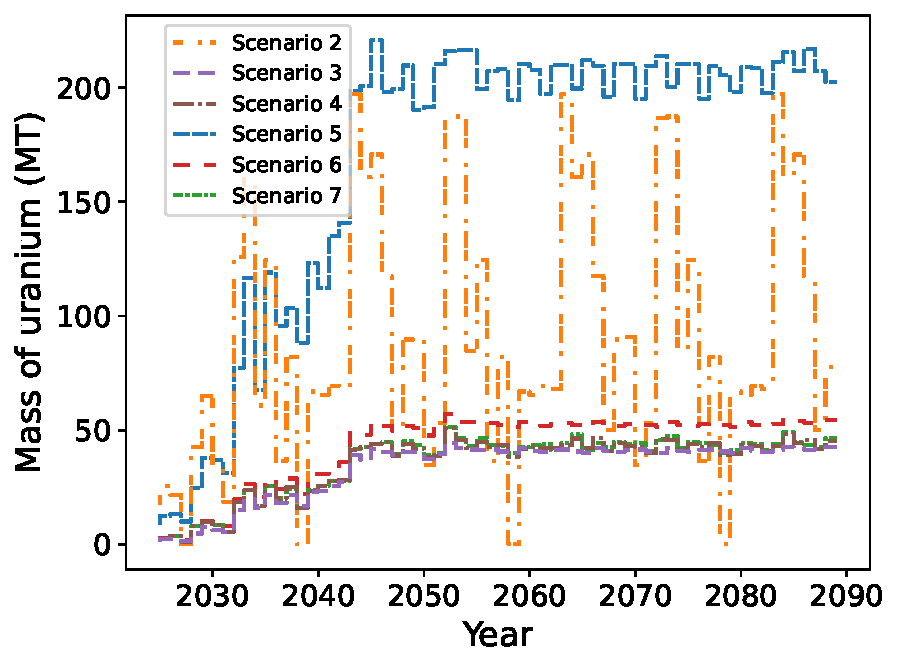
\includegraphics[scale=0.43]{nogrowth_AR_uranium.pdf}
                \caption{Annual average mass of enriched uranium required to fuel
                advanced reactors in Scenarios 2-7.}
                \label{fig:uranium}

        \end{figure}
    \end{columns}
\end{frame}

\begin{frame}
    \frametitle{\gls{SNF} discharged follows with fuel mass}
    \begin{columns}
        \column[t]{4.3cm}
            \begin{itemize}
                \item Scenario 5 (MMR + VOYGR) discharges the largest mass of \gls{SNF}
                \item Scenario 3 (Xe-100) discharges the least \gls{SNF}
                \item Scenario 2 (MMR) discharges \gls{SNF} the latest
                \item Cumulative masses range between 25,654 MT (Scenario 3) to 
                      112,913 MT (Scenario 5)
                
            \end{itemize}
        \column[t]{5.7cm}
        \vspace{-1cm}
        \begin{figure}
                \centering
                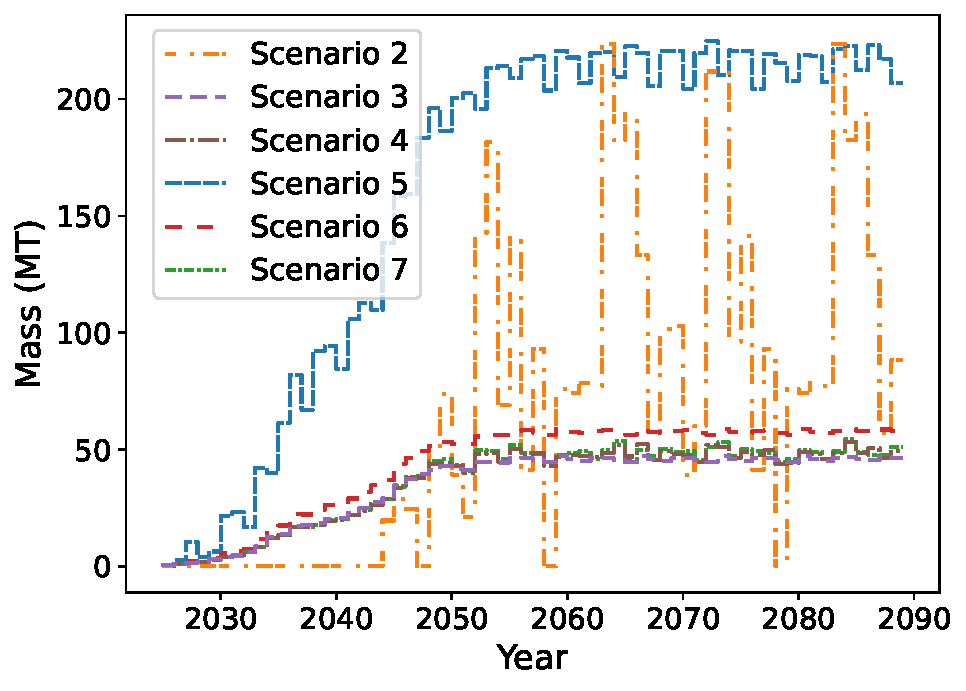
\includegraphics[scale=0.43]{nogrowth_AR_waste.pdf}
                \caption{Annual average mass of \gls{SNF} discharged from 
                advanced reactors in Scenarios 2-7.}
                \label{fig:waste}
        \end{figure}
    \end{columns}
\end{frame}
\section{Sensitivity analysis \& Optimization}
\subsection{Sensitivity analysis}
\begin{frame}
    \frametitle{Sensitivity analysis provides more insight into 
    the fuel cycles.}
    To meet the third objective, I perform sensitivity analysis 
    on Scenario 7, comparing the impact of different model parameters
    \begin{itemize}
        \item Couple \Cyclus with Dakota \cite{adams_dakota_2021}
        \item Parameters include:
        \begin{itemize}
            \item Transition start time
            \item Percent of \glspl{LWR} operating for 80 years
            \item Build share of Xe-100, VOYGR, MMR
            \item Discharge burnup of Xe-100 and MMR
        \end{itemize}
        \item Vary these parameters individually
        \item Vary these parameters in different combinations
    \end{itemize}

\end{frame}

\begin{frame}
    \frametitle{Varying the Xe-100 build share has a mixed effect}
    \begin{columns}

        \column[t]{4.5cm}
        \begin{itemize}
            \item HALEU-related metrics all increase
            \item Total fuel mass and the SNF mass decrease
            \item Total SWU capacity is relatively constant
            \item Results are a function of the number of
                  each advanced reactor deployed
        \end{itemize}

    \column[t]{5.5cm}
    \begin{figure}
        \centering 
            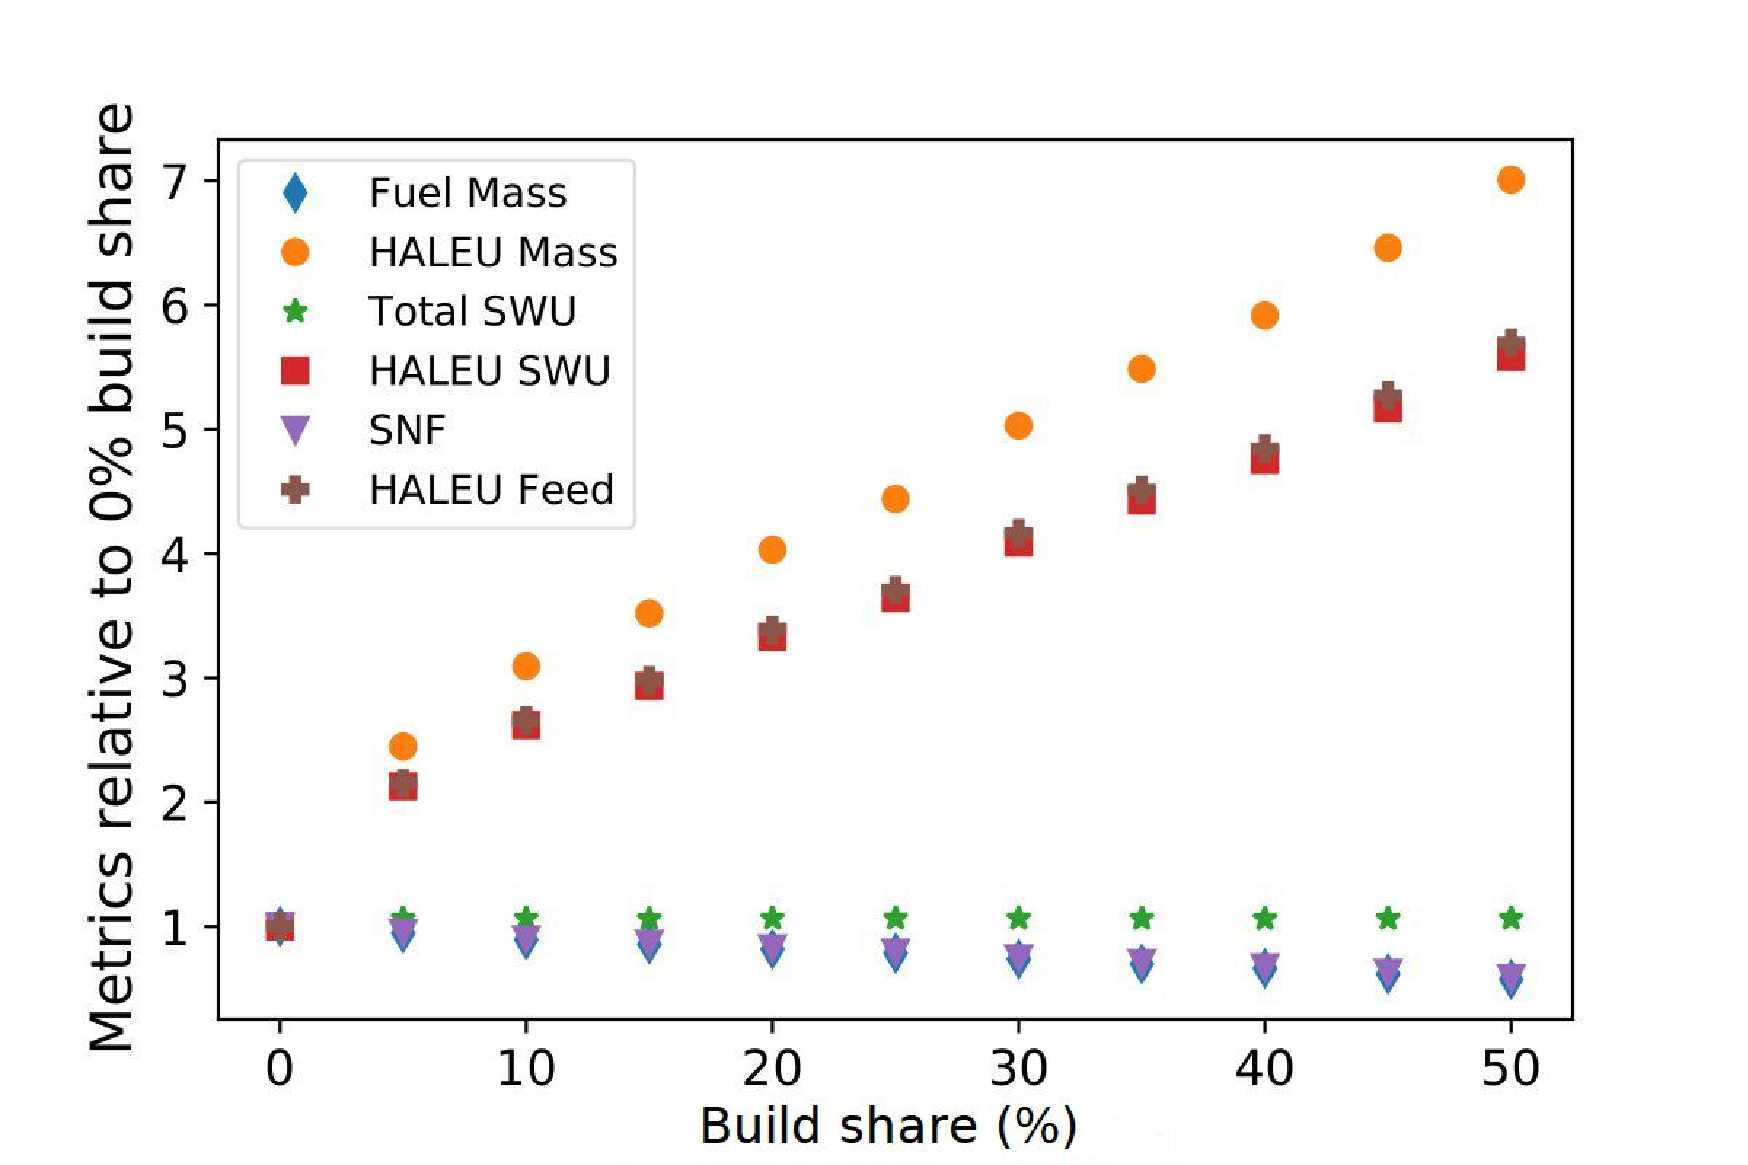
\includegraphics[scale=0.4]{xe100.pdf}
            \caption{Relative effect of varying Xe-100 build share}
            \label{fig:xe100_effects}
    \end{figure}

\end{columns}
\end{frame}

\begin{frame}
    \frametitle{Effects of varying Xe-100 build share}
    \begin{figure}
        \centering
        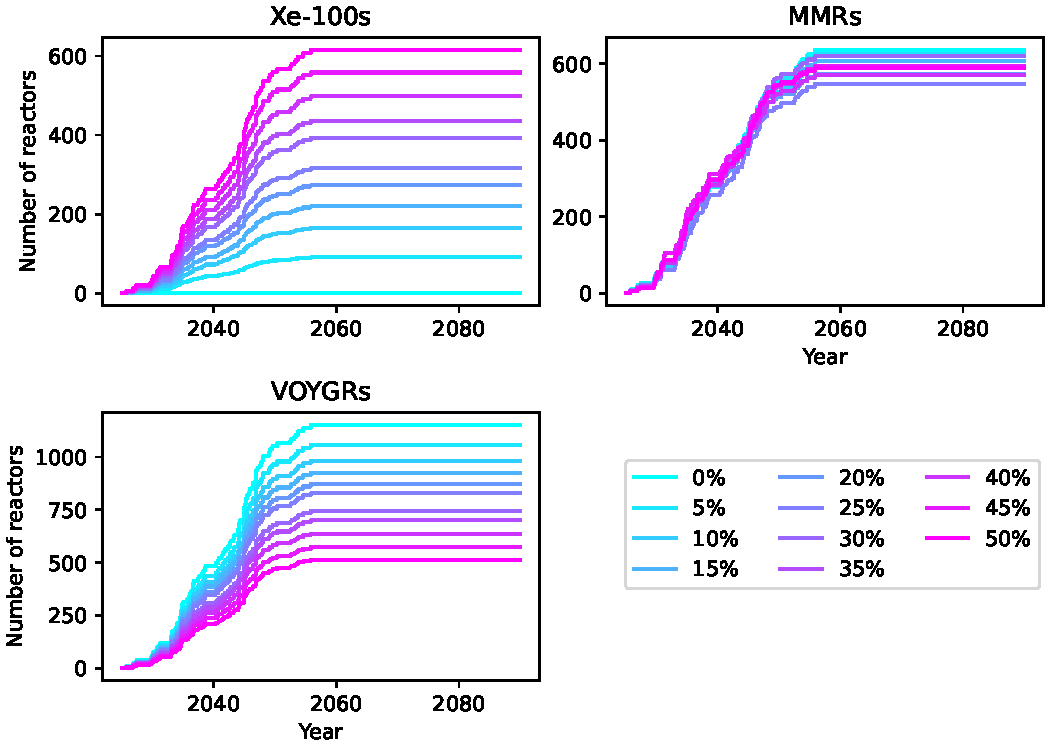
\includegraphics[scale=0.5]{xe100_combined_reactors.pdf}
        \caption{Number of Xe-100s (top left), MMRs (top right), and VOYGRs
        (bottom left) as a function of Xe-100 build share.}
        \label{fig:xe100_s7_combined_reactors}
    \end{figure}
\end{frame}

\begin{frame}
    \frametitle{Effects of varying Xe-100 and MMR burnup}
    \begin{columns}

        \column[t]{4cm}
        \begin{itemize}
            \item Non-uniform relationship
            \item At smaller Xe-100 burnup values the increasing MMR 
                  share decreases the HALEU mass
            \item At larger Xe-100 burnup values the increasing MMR share 
                  increases the HALEU mass
            \item Comparison of how much fuel each reactor needs
        \end{itemize}

    \column[t]{6cm}
    \vspace{-1cm}
    \begin{figure}
        \centering 
            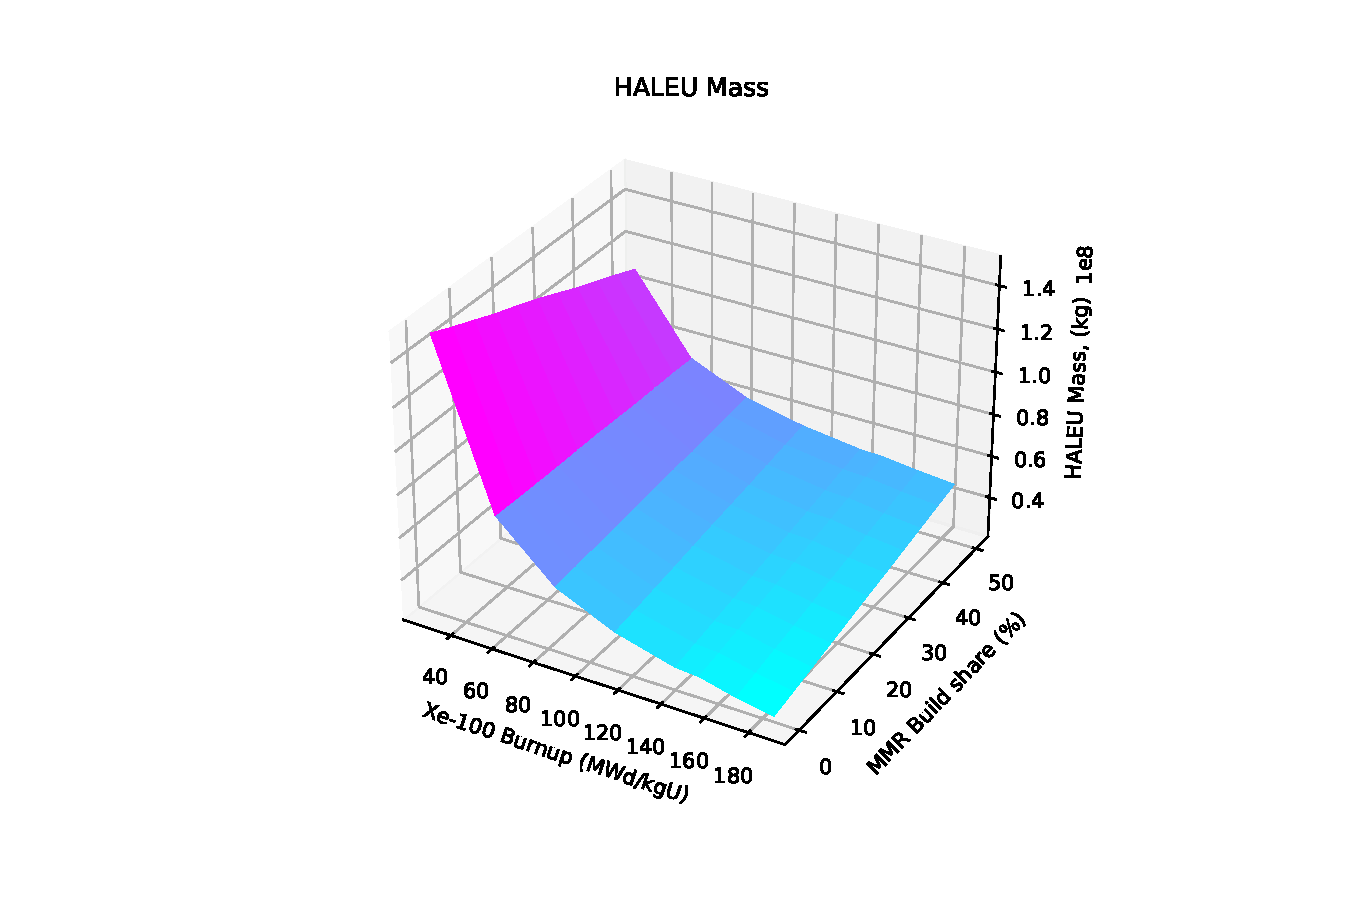
\includegraphics[scale=0.5, trim=180 45 70 50,clip]{mmr_share_xe100_burnup_haleu.pdf}
            \caption{Effects of varying the MMR build share and 
            Xe-100 discharge burnup on HALEU mass}
            \label{fig:mmr_share_xe100_bu}
    \end{figure}

\end{columns}
\end{frame}

\begin{frame}
    \frametitle{Varying multiple parameters shows importance of the 
    Xe-100 burnup}
    \begin{table}
        \centering
        \caption{Sobol' indices for the Gaussian model when varying the 
        Xe-100 build share. Highlighted 
        values indicate a total Sobol' indices of above 0.5.}
        \label{tab:s7_sobol_xe100_gaussian}
        \begin{tabular}{c c c c c c c}
            \hline
            & \multicolumn{6}{c}{Output Metric} \\
            Parameter & Fuel Mass & HALEU Mass & SWU & HALEU SWU & Feed & SNF Mass \\
            \hline
            Transition Start & 0.003 & 0.007 & 0.009 &
                               0.009 & 0.009 & 0.003\\
            LWR Lifetime & 0.280 & 0.021 & 0.095 &
                           0.022 & 0.022 & 0.314\\
            Xe-100 Share & \cellcolor{green!25}0.533 & \cellcolor{green!25}0.513 & 0.283 &
            \cellcolor{green!25}0.511 & \cellcolor{green!25}0.512 & 0.474\\
            Xe-100 Burnup & 0.247 & \cellcolor{green!25}0.571 & \cellcolor{green!25}0.775 & 
            \cellcolor{green!25}0.568 & \cellcolor{green!25}0.568 & 0.280\\
            MMR Burnup & 0.002 & 0.004 & 0.006 & 
                         0.005 & 0.005 & 0.002\\
            \hline        
        \end{tabular}
    \end{table}
        %<2-> \tikz[overlay, remember picture]{\draw{draw=red,thick, double, fillopacity=0.2] ($(infrastructure)+(-0.5,0.4)$) rectangle ($(infrastructure)+(6,-0.2)$);}} 
\end{frame}

\subsection{Optimization}
\begin{frame}
    \frametitle{Use the \Cyclus-Dakota coupling to optimize the transition}
    \begin{itemize}
        \item Use the Genetic algorithm in Dakota (single-objective or 
        multi-objective) to perform optimization.
        \item Use the parameters considered for sensitivity analysis, 
              except the transition start time
        \item Apply a linear constraint for the advanced reactor build shares
        \item Goal is to minimize the SWU capacity needed to 
             produce HALEU, the mass of SNF, or both
    \end{itemize}
\end{frame}

\begin{frame}
    \frametitle{Multi-objetive optimization isn't perfect}
    \begin{columns}
        \column[t]{5cm}
        \begin{itemize}
            \item Optimizing for these metrics is a trade-off between 
                 building Xe-100s and VOYGRs
            \item Genetic algorithm struggles with linear constraint for 
                  the three build shares
        \end{itemize}

        \column[t]{5cm}
        \begin{figure}
            \centering 
            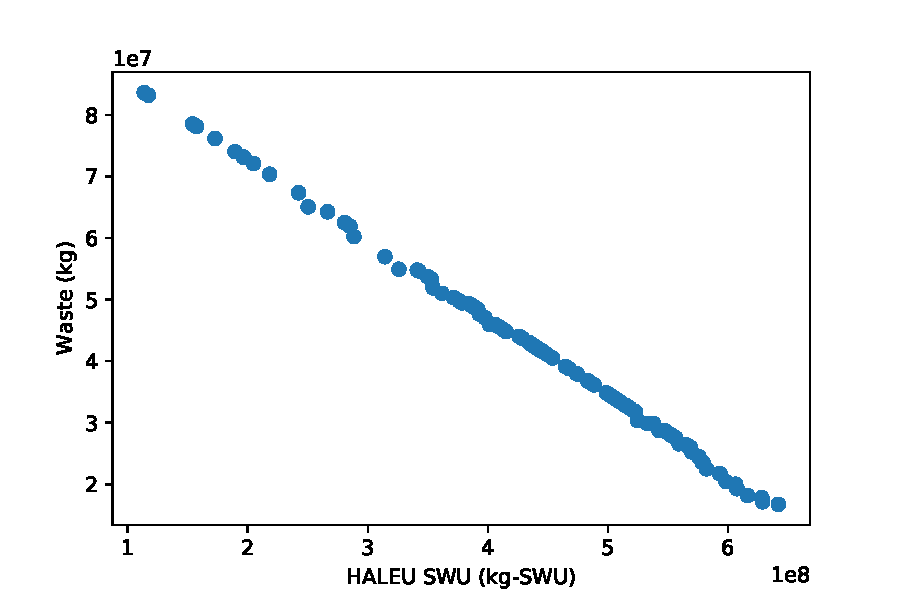
\includegraphics[scale=0.4]{once_through_pareto.pdf}
            \caption{Pareto front for multi-objective optimization}
            \label{fig:pareto}
        \end{figure}
    \end{columns}
    
\end{frame}
\section{Effects of impurities}
\begin{frame}
    \frametitle{Downblending HEU is a potential source of HALEU}
    To meet the fourth objective, I modeled the neutronics of 
    different HALEU compositions in the Xe-100 and MMR.
    \begin{itemize}
        \item Consider pure HALEU ($^{235}$U and $^{238}$U only)
              and HALEU from downblended \gls{EBR} 
              \cite{vaden_isotopic_2018} and Y-12 
              \cite{nelson_foreign_2010} stockpiles
        \item Create models in Serpent \cite{leppanen_serpent_2013} 
              for these two reactors
        \item Compare the performance of the fuels with respect to:
        \begin{itemize}
            \item \keff
            \item \betaEff
            \item Energy- and spatially-dependent flux
            \item Fuel, coolant, moderator, and total reactivity
                  temperature feedback coefficients
        \end{itemize}
    \end{itemize}

\end{frame}

\begin{frame}
    \frametitle{\keff and \betaEff of Xe-100}
    \begin{columns}
        \column[t]{5cm}
    \begin{itemize}
        \item Impurities increase \keff, larger $\eta$ value of the fuel 
        \item<2-> Impurities decrease \betaEff because non$^{235}$U 
              isotopes have a smaller \betaEff than $^{235}$U
    \end{itemize}
        \column[t]{5cm}
        \begin{table}[ht]
            \centering 
            \caption{\keff values for the Xe-100-like reactor model using
            each fuel type.}
            \label{tab:xe100_keff}
            \begin{tabular}{c c}
                    \hline
                    Fuel type & \keff \\
                    \hline 
                    Pure & 1.06663 $\pm$ 0.00016\\
                    \gls{EBR} & 1.08086 $\pm$ 0.00016\\
                    Y-12 & 1.08016 $\pm$ 0.00014\\
                    \hline                
            \end{tabular}
        \end{table}

        \pause
        \begin{table}[ht]
            \centering 
            \caption{\betaEff value for the Xe-100-like reactor 
            mode using each fuel type.}
            \label{tab:betaeff_xe100}
            \begin{tabular}{c c}
                    \hline
                    Fuel type & \betaEff \\
                    \hline
                    Pure & 0.00617 $\pm$ 0.00003 \\
                    \gls{EBR} & 0.00604 $\pm$ 0.00003 \\
                    Y-12 & 0.00598 $\pm$ 0.00003 \\
                    \hline
            \end{tabular}
        \end{table}
    \end{columns}

\end{frame}

\begin{frame}
    \frametitle{Energy dependent neutron flux in Xe-100}
    \begin{figure}
        \centering 
        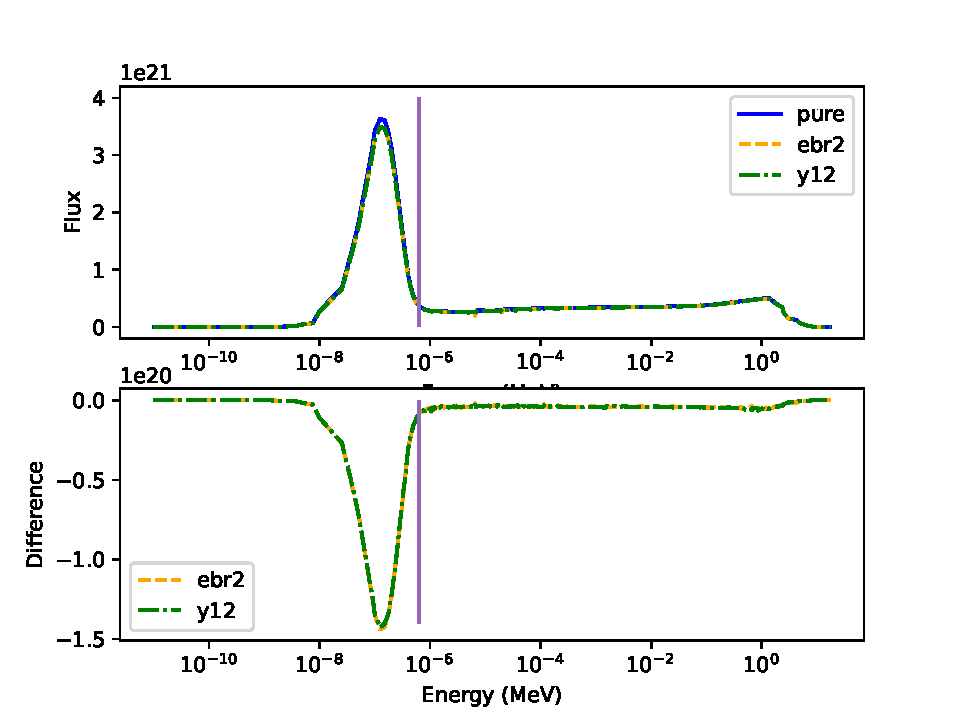
\includegraphics[scale=0.5]{xe100_mg_flux.pdf}
        \caption{Energy-dependent flux through the active region 
        of the Xe-100 core. The purple line is the delineation 
        between fast and thermal neutrons for this work.}
    \end{figure}
\end{frame}

\begin{frame}
    \frametitle{Spatitally-dependent neutron flux in Xe-100}
    \begin{figure}
        \centering 
        \begin{subfigure}{0.49\textwidth}
            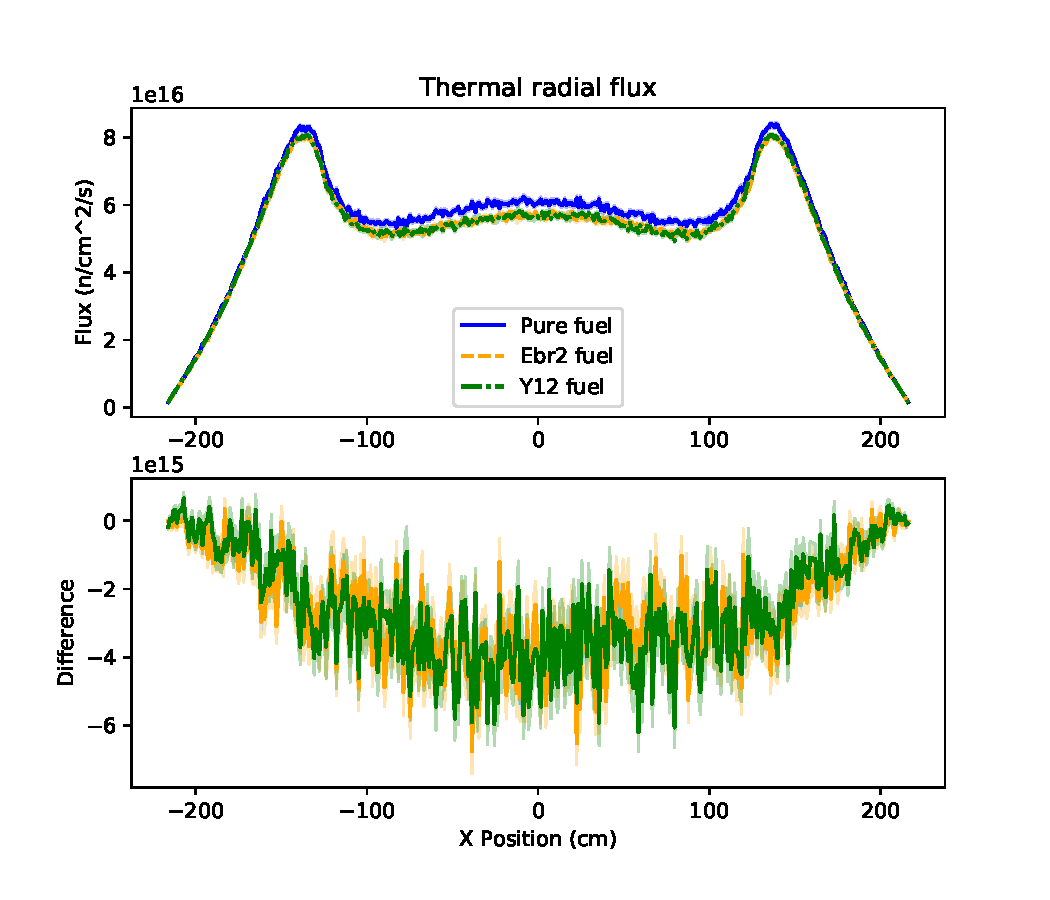
\includegraphics[scale=0.35, trim=20 10 10 20,clip]{xe100_thermal_radial.pdf}
        \end{subfigure}
        \begin{subfigure}{0.49\textwidth}
            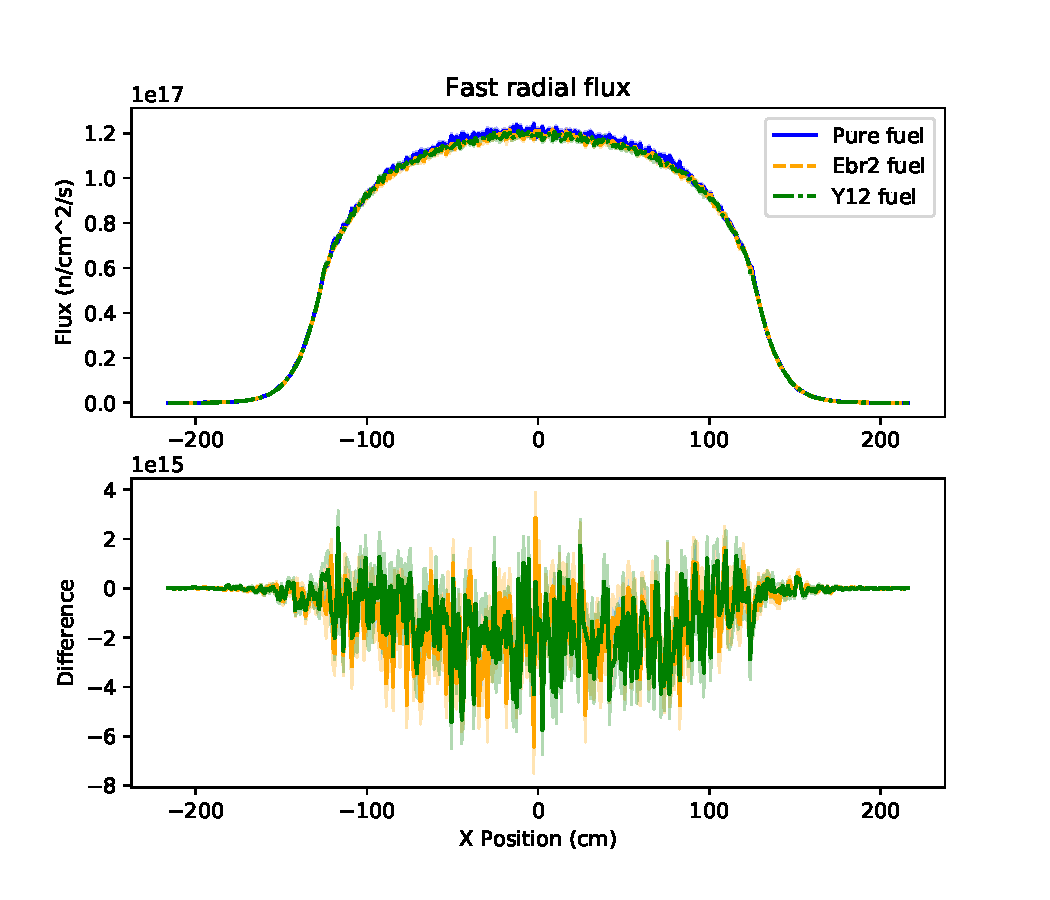
\includegraphics[scale=0.35, trim=10 10 10 20,clip]{xe100_fast_radial.pdf}
        \end{subfigure}
        \caption{Radial fluxes through Xe-100.}
        \label{fig:xe100-flux}
    \end{figure}
\end{frame}
\section{Conclusions}
\begin{frame}
      \frametitle{Conclusions}
      \begin{itemize}
        \item This work investigates the impacts of deploying \gls{HALEU}-fueled 
              reactors on the nuclear fuel cycle.
        \item<2-> The material requirements of the transitions modeled are governed 
              by the design characteristics of the reactors deployed
        \item<2-> Closing the fuel cycle decreases material needs, but the 
              decrease is governed by the recycling scheme and the 
              material available for reprocessing
        \item<3-> Sensitivity analysis showed more details on how the 
              advanced reactor characteristics affect the material requirements, and 
              the importance of the Xe-100 burnup
        \item<3-> Found optimized transitions, but other algorithms should 
              be used when using a linear constraint
        \item<4-> The impurities from downblending \gls{HEU} affect 
              reactor parameters, but won't necessarily prevent key design 
              parameters from being met
      \end{itemize}
\end{frame}

\begin{frame}
      \frametitle{Limitations and Future Work}
      \begin{itemize}
            \item Transition analysis provided a macroscopic view of 
                  material needs, focused on fuels
            \begin{itemize}
                  \item<2-> Model the needs of non-fuel materials, 
                        like reactor-grade graphite
                  \item<2-> Determine and model facility capacities
                  \item<2-> Account for processing time 
            \end{itemize}
            \item<3-> Ignores other externalities, like nonproliferation
                    safeguards
            \begin{itemize}
                  \item<4-> Incorporate potential safeguards measures into models
            \end{itemize}
            \item<5-> Expand analysis on impurities in \gls{HALEU}
            \begin{itemize}
                  \item<6-> Consider power-peaking factors
                  \item<6-> Model burnable poisons and control rods 
                  \item<6-> Model core in non-isothermal state
            \end{itemize}
      \end{itemize} 
\end{frame}
\begin{frame}
    \frametitle{Acknowledgements}
    \begin{itemize}
        \item This material is based upon work supported under a University 
        Nuclear Leadership Program Graduate Fellowship. Any opinions, findings, conclusions, or 
    recommendations expressed in this publication are those of the author(s) 
    and do not necessarily reflect the views of the Department of Energy Office 
    of Nuclear Energy.
        \item Grainger College of Engineering for providing me with
              a SURGE Fellowship
        \item Committee Members
        \item ARFC Group members
        \item RFCA members, Drs. Bo Feng and Scott Richards
        \item \Cyclus and OpenMC communities
        \item Kyle and Little R
    \end{itemize}
\end{frame}



\begin{frame}[allowframebreaks]
    \frametitle{References}
    \bibliographystyle{plain}
    {\footnotesize \bibliography{../bibliography} }
  
\end{frame}

\begin{frame}
    \centering
    
\includegraphics[scale=0.25,trim=0 600 0 700,clip]{LittleR.jpg}
\end{frame}

\begin{frame}
    \frametitle{More limitations and future work}
    \begin{itemize}
    \item Ignores other externalities, like nonproliferation
        safeguards
    \begin{itemize}
        \item Incorporate potential safeguards measures into models
        \item Account for construction time and/or licensing
    \end{itemize}
    \item Expand analysis on impurities in \gls{HALEU}
    \begin{itemize}
        \item Consider power-peaking factors
        \item Model burnable poisons and control rods 
        \item Model core in non-isothermal state
    \end{itemize}
\end{itemize}
\end{frame}

\begin{frame}
    \frametitle{Once-through feed uranium}
    \begin{figure}
        \centering 
        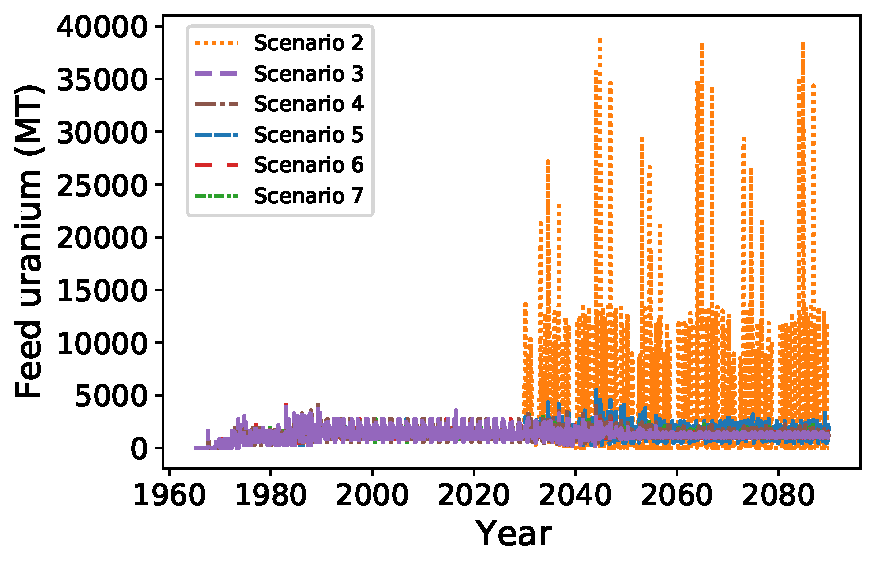
\includegraphics[scale=0.5]{nogrowth_feed.pdf}
    \end{figure}
\end{frame}

\begin{frame}
    \frametitle{Recycle HLW}
    \begin{figure}
        \centering
        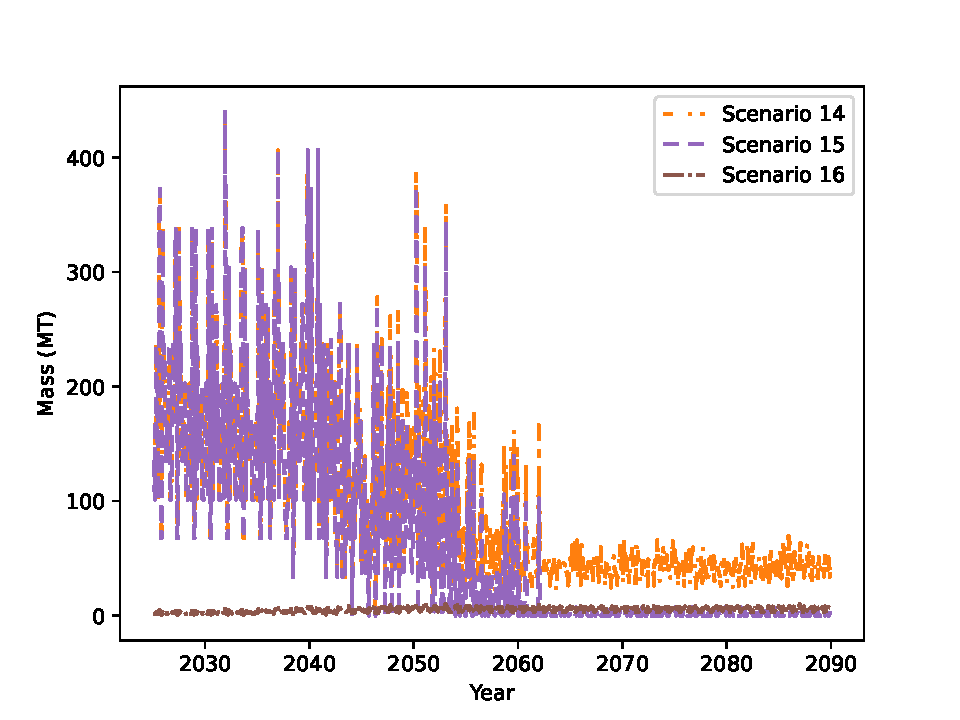
\includegraphics[scale=0.5]{nogrowth_recycle_hlw.pdf}
    \end{figure}
\end{frame}

\begin{frame}
    \frametitle{Recycle SNF}
    \begin{figure}
        \centering
        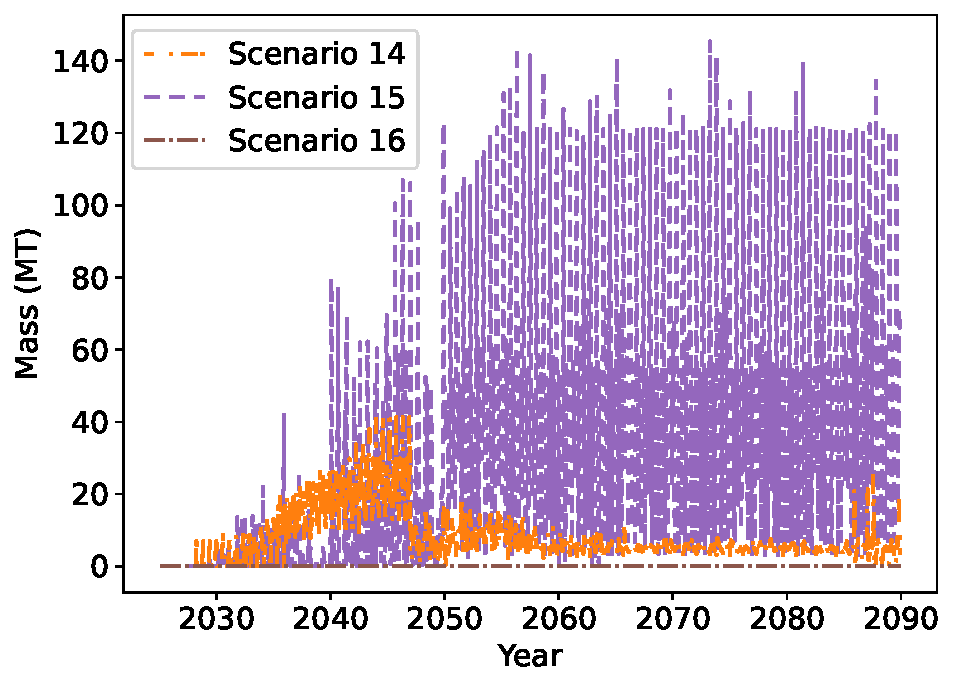
\includegraphics[scale=0.5]{nogrowth_recycle_snf.pdf}
    \end{figure}
\end{frame}

\begin{frame}
    \frametitle{Recycle SWU}
    \begin{figure}
        \centering
        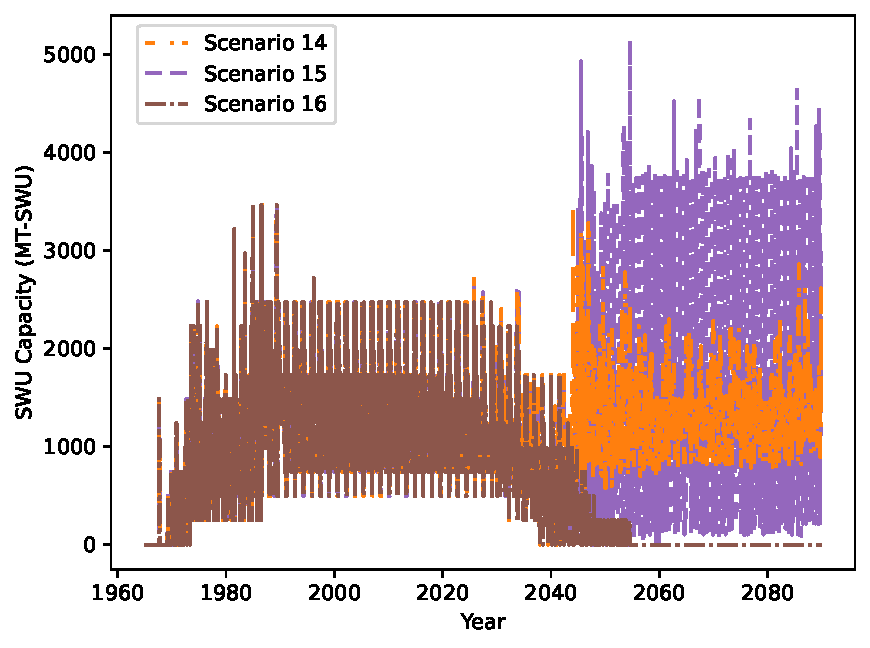
\includegraphics[scale=0.5]{nogrowth_recycle_swu.pdf}
    \end{figure}
\end{frame}

\begin{frame}
    \frametitle{Effects of varying VOYGR build share}
    \begin{figure}
        \centering
        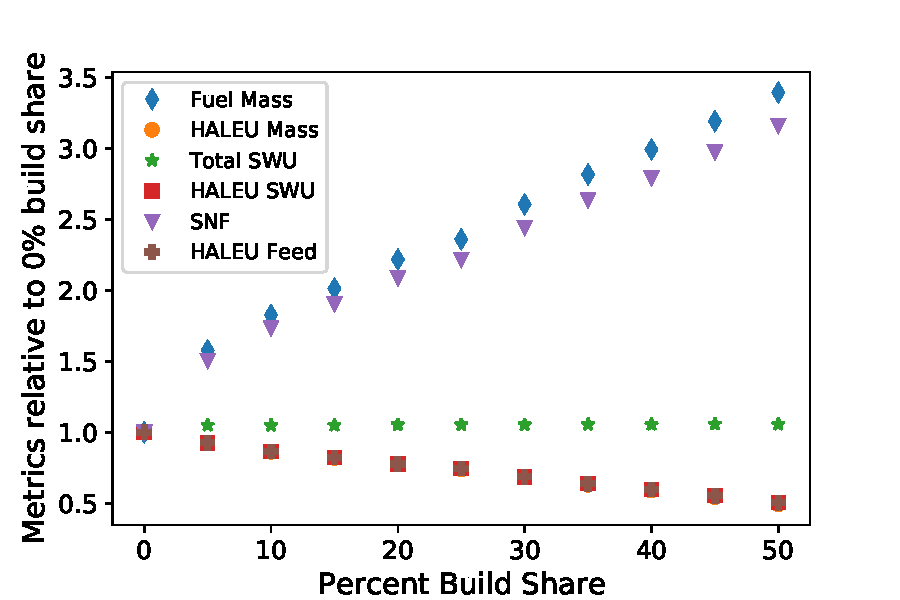
\includegraphics[scale=0.3]{voygr.pdf}
    \end{figure}
\end{frame}

\begin{frame}
    \frametitle{Effects of varying Xe-100 build share}
    \begin{figure}
        \centering
        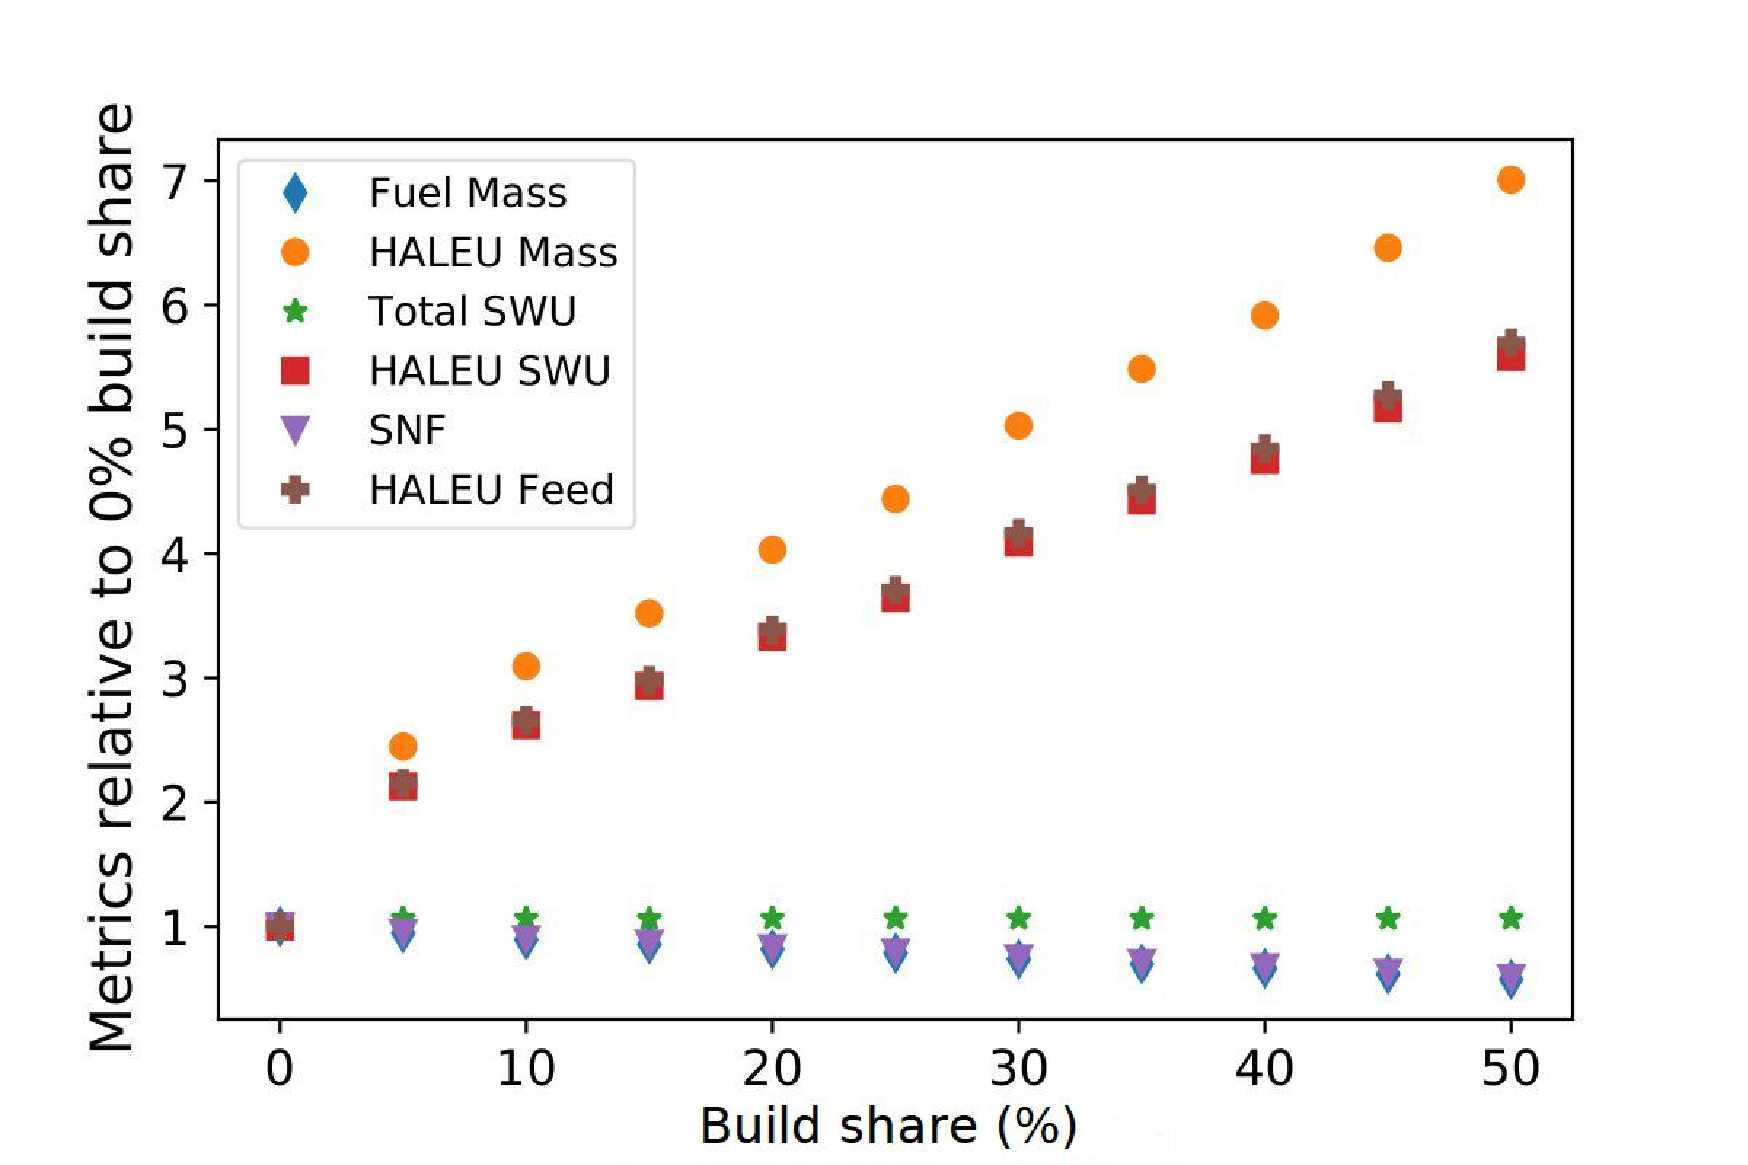
\includegraphics[scale=0.3]{xe100.pdf}
    \end{figure}
\end{frame}
\begin{frame}
    \frametitle{Effects of varying LWR lifetimes}
    \begin{figure}
        \centering
        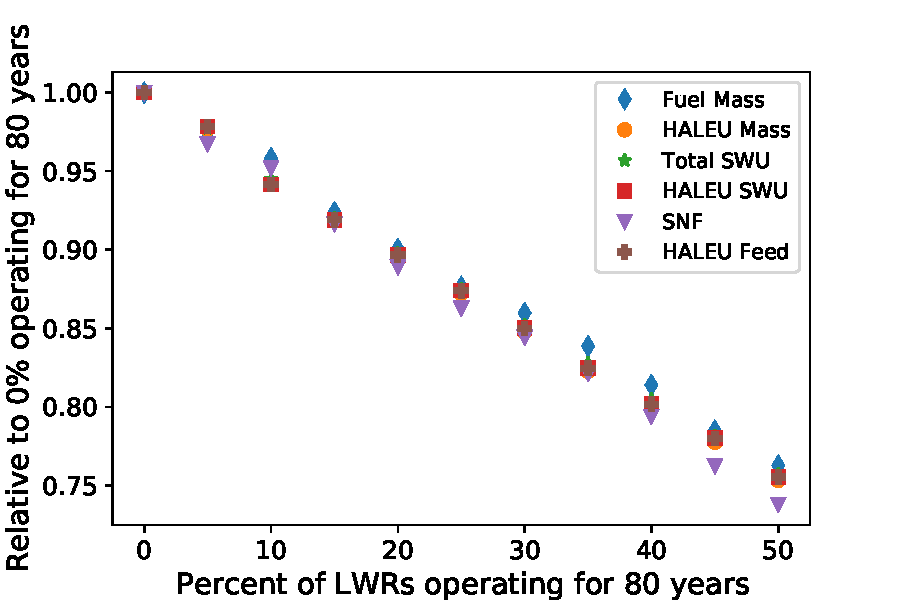
\includegraphics[scale=0.5]{lwr.pdf}
    \end{figure}
\end{frame}
\begin{frame}
    \frametitle{Effects of varying transition start time}
    \begin{figure}
        \centering
        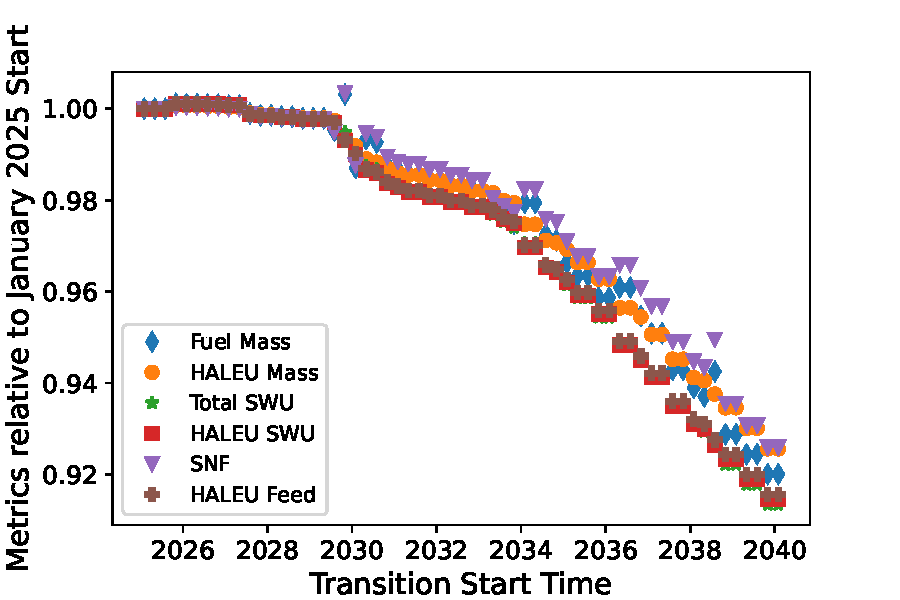
\includegraphics[scale=0.5]{ts.pdf}
    \end{figure}
\end{frame}

\begin{frame}
    \frametitle{HALEU SWU Optimization}
    
\begin{table}[h!]
    \centering 
    \caption{Values resulting in a minimum \gls{HALEU} \gls{SWU} capacity for 
              a once-through transition scenario.}
    \label{tab:soga_ot_haleu}
    \begin{tabular}{c c}
        \hline
        Variable & Value \\
        \hline
        LWR Lifetime & 36\%\\
        Xe-100 build share & 0\%\\
        MMR build share & 2\%\\
        VOYGR build share & 100\%\\
        Xe-100 burnup & 151 MWd/kgU\\
        MMR burnup & 90 MWd/kgU\\
        \hline
        HALEU SWU & 4.812 $\times 10^7$ kg-SWU\\
        \hline
    \end{tabular}
\end{table}
    
\end{frame}

\begin{frame}
    \frametitle{Axial flux through Xe-100}
    \begin{figure}
        \centering 
        \begin{subfigure}{0.49\textwidth}
            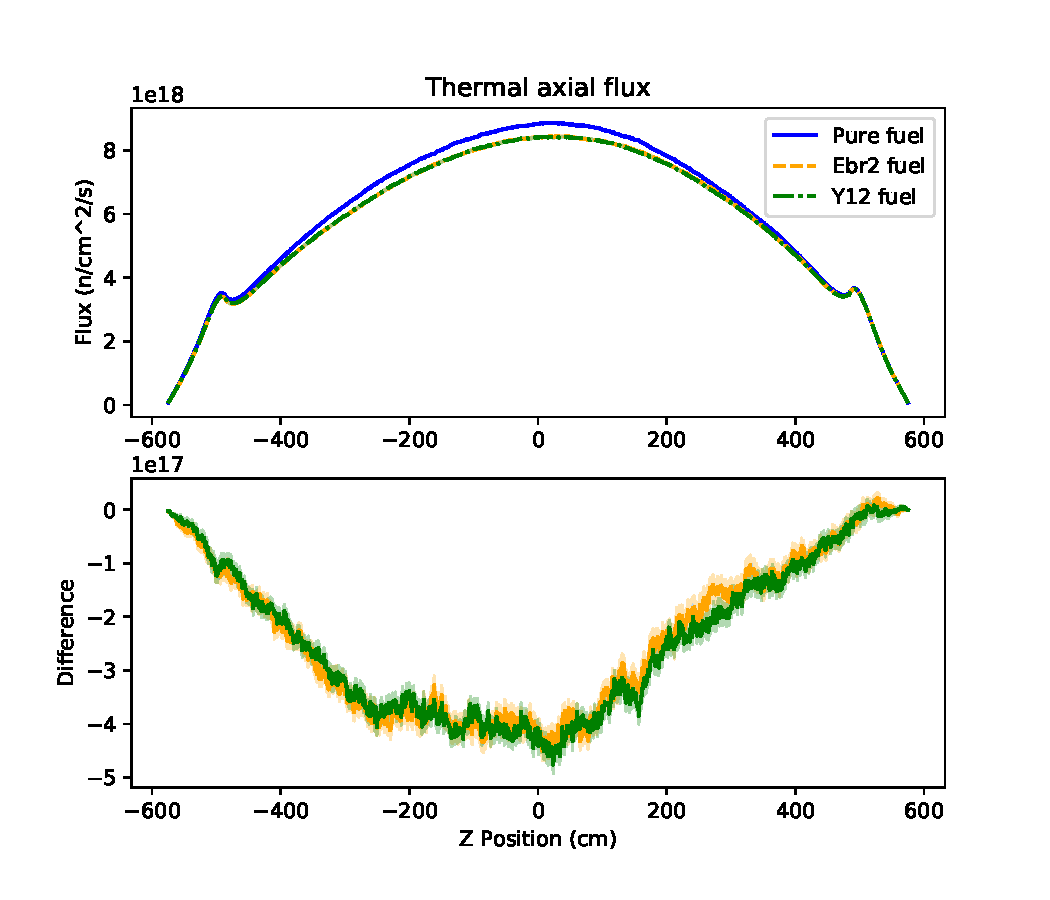
\includegraphics[scale=0.35, trim=20 10 10 20,clip]{xe100_thermal_axial.pdf}
        \end{subfigure}
        \begin{subfigure}{0.49\textwidth}
            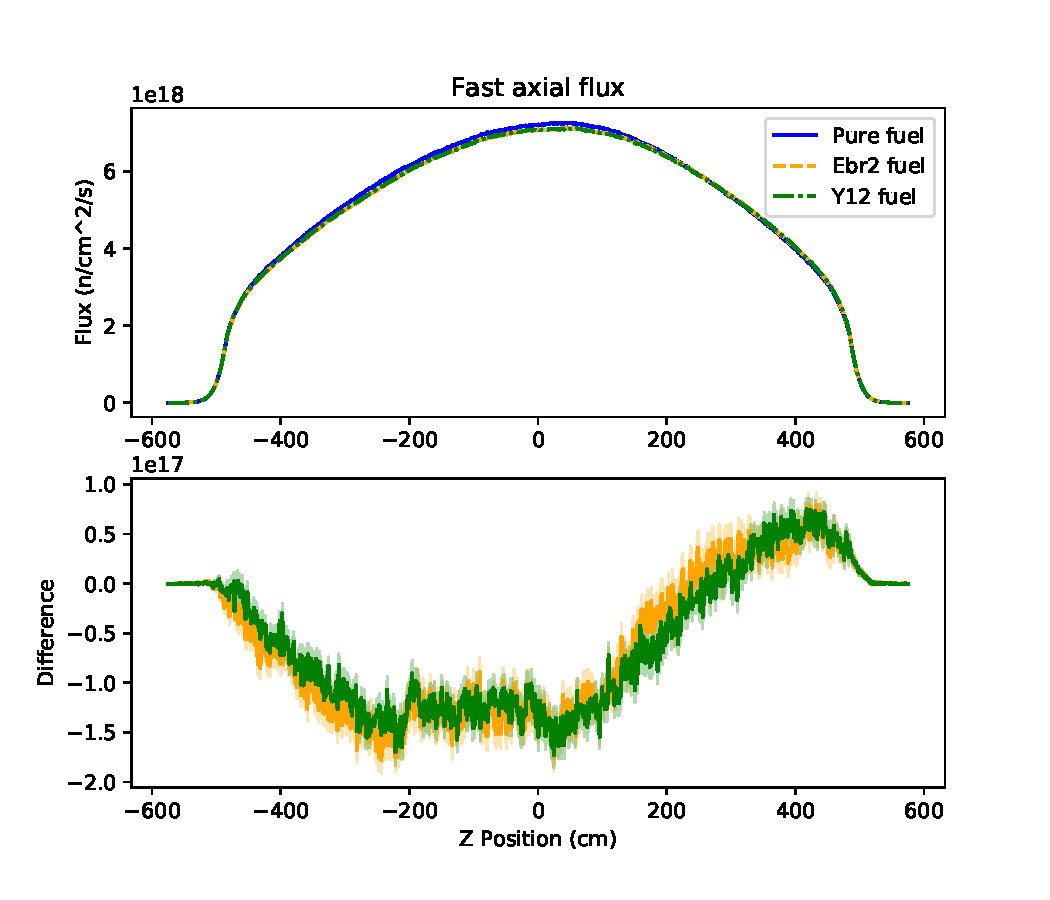
\includegraphics[scale=0.35, trim=10 10 10 20,clip]{xe100_fast_axial.pdf}
        \end{subfigure}
        \caption{Axial fluxes through Xe-100.}
        \label{fig:xe100-axial-flux}
    \end{figure}
\end{frame}

\begin{frame}
    \frametitle{Reactivity feedback coefficients for Xe-100}
    \begin{table}[ht]
        \centering
        \caption{Reactivity temperature feedback coefficients for 
        each material type in the Xe-100-like model for each fuel 
        type.}
        \label{tab:coeff_xe100}
        \begin{tabular}{c c c c c}
            \hline 
            & \multicolumn{4}{c}{Material feedback coefficient (pcm/K)} \\
            Fuel Type & Fuel & Coolant & Moderator & Total \\
            \hline
            Pure & -3.875 $\pm$ 0.094 & -0.044 $\pm$ 0.112 & -0.071 $\pm$ 0.459 & -4.216 $\pm$ 0.502\\
            \gls{EBR} & -3.759 $\pm$ 0.138 & -0.433 $\pm$ 0.048 & -0.708 $\pm$ 0.404 & -4.817 $\pm$ 0.438\\
            Y-12 & -3.797 $\pm$ 0.157 & -0.351 $\pm$ 0.092 & -0.728 $\pm$ 0.469 & -4.700 $\pm$ 0.349\\
            \hline

        \end{tabular}
\end{table}
\end{frame}

\end{document}
